\documentclass[10pt,journal,compsoc]{IEEEtran}

\usepackage{amsmath,amssymb,amsfonts,amsthm}
\usepackage{graphicx}
\usepackage{booktabs}
\usepackage{multirow}
\usepackage{array}
\usepackage{cite}
\usepackage{xcolor}
\usepackage{algorithm}
\usepackage{algorithmic}

\newtheorem{proposition}{Proposition}
\newtheorem{remark}{Remark}

\hyphenation{op-tical net-works semi-conduc-tor post-quan-tum homo-mor-phic}

\usepackage[hidelinks]{hyperref}

\begin{document}

\title{CAPQ-Pareto: SLA-Aware Causal Bandit Orchestration of Post-Quantum Transport, SIMD Homomorphic Encryption, and Hybrid Vector Databases Across the Cloud--Edge Continuum}

\author{Preecha~Noiumkar,~\IEEEmembership{Member,~IEEE}%
\IEEEcompsocitemizethanks{\IEEEcompsocthanksitem P. Noiumkar is with the Department of Information Technology, Faculty of Informatics, Mahasarakham University, Maha Sarakham 44150, Thailand (e-mail: preecha.n@msu.ac.th; ORCID: \protect\protect\url{https://orcid.org/0009-0000-5964-4896}).\protect\\
Corresponding author: Preecha Noiumkar (e-mail: preecha.n@msu.ac.th).}%
\thanks{This research project was financially supported by the Faculty of Informatics, Mahasarakham University. Reproducible V2 Artifacts and SHA-256 Telemetry Logs: \protect\url{https://github.com/preecha-msu/CAPQ-Pareto}.}}

\markboth{IEEE TRANSACTIONS ON CLOUD COMPUTING}%
{NOIUMKAR: CAPQ-PARETO NON-STATIONARY BANDIT ORCHESTRATION ACROSS THE CLOUD-EDGE CONTINUUM}

\IEEEtitleabstractindextext{%
\begin{abstract}
Transitioning cloud-edge data planes to post-quantum cryptography (PQC) and confidential retrieval-augmented generation introduces coupled bottlenecks across wide-area network (WAN) transport, homomorphic compute, and approximate nearest-neighbor indexing. Unpooled TLS 1.3 handshakes carrying ML-KEM key shares and ML-DSA certificate chains trigger multi-MTU head-of-line stalls under packet loss, whereas single-probe Ring-LWE homomorphic search suffers cluster-boundary recall degradation. Moreover, claiming deterministic latency guarantees across intercontinental routes contradicts physical propagation floors. We present CAPQ-Pareto, an empirical SLA-aware causal bandit orchestrator governed by a stabilized Discounted LinUCB controller operating strictly on lagged pre-decision telemetry with zero future leakage. CAPQ-Pareto formalizes a Three-Tier Bounded SLA Architecture: a hard pre-execution gate enforcing calibrated Recall@10 of at least 0.92 and zero-trust CKKS via SPANN boundary replication with pre-encoded SIMD RNS buckets; soft predictive latency filtering with 60-ms timeout fallback; and dual-class empirical SLA auditing across 150-ms regional interactive and 350-ms cross-continent analytical tiers. Validated on 1,000,000-vector SIFT1M and 100,000-vector BGE-M3 corpora, a 32-run factorial ANOVA, unseen WAN shocks, 10,000-query quantization audits, adversarial leakage tests, and 1,800 live three-region Google Cloud transactions, CAPQ-Pareto achieves 93.75\% to 100\% unweighted 4D Pareto frontier occupancy.
\end{abstract}

\begin{IEEEkeywords}
Cloud-edge continuum, post-quantum cryptography, ML-KEM, ML-DSA, CKKS homomorphic encryption, vector databases, HNSW, non-stationary contextual bandits, Pareto optimization.
\end{IEEEkeywords}}

\maketitle
\IEEEdisplaynontitleabstractindextext
\IEEEpeerreviewmaketitle

\section{Introduction}
\IEEEPARstart{M}{odern} cloud-edge applications increasingly interleave transactional relational queries, semi-structured JSON document lookups, high-dimensional semantic vector search for retrieval-augmented generation (RAG), and privacy-preserving confidential similarity queries within unified application streams~\cite{pan2024vectordbsurvey,chen2024bgem3}. Securing these heterogeneous data planes against harvest-now-decrypt-later adversaries requires migrating transport protocols to NIST-standardized post-quantum key encapsulation (FIPS~203 ML-KEM~\cite{nist_fips203_2024}) and digital signatures (FIPS~204 ML-DSA~\cite{nist_fips204_2024}), while protecting sensitive tenant queries against untrusted cloud operators demands fully homomorphic encryption (FHE) such as Cheon--Kim--Kim--Song (CKKS)~\cite{cheon2017ckks,albadawi2022openfhe}.

Deploying these primitives naively across mobile and wide-area cloud-edge links exposes three compounding systems pathologies that are obscured in isolated microbenchmarks:
\begin{enumerate}
    \item \textbf{Handshake Amplification vs. Connection Pooling:} While unpooled TLS~1.3 handshakes carrying ML-KEM-768/1024 key shares and full three-certificate ML-DSA-65 authentication chains ($11,879$~bytes of signature/key material alone, spanning $9$ Ethernet frames) suffer severe multi-RTT head-of-line (HoL) stalls under packet loss~\cite{paquin2020pqctls,sosnowski2023pqckem}, production database drivers amortize handshake overhead via persistent connection pools and RFC~8446 session tickets~\cite{rfc8446_tls13}. Fair evaluation therefore requires benchmarking adaptive transport orchestration directly against \emph{warm, persistent hybrid PQC TLS~1.3 pools}, isolating true transport-layer HoL blocking on multi-MTU payloads from artificial per-query TCP/TLS setup overhead.
    \item \textbf{The Single-Probe Confidential Recall Ceiling:} Exhaustive homomorphic inner-product evaluation over million-scale corpora is latency-prohibitive. Partitioning encrypted enclave vectors into $K_c$ disjoint Voronoi clusters and probing only $r=1$ nearest centroid keeps latency low, but boundary queries miss true top-$K$ neighbors residing in adjacent cells. In streams containing $75\%$ plaintext relational/vector queries and $25\%$ zero-trust confidential queries, disjoint single-probe CKKS caps overall SLA compliance at $\approx 75.0\%$ regardless of transport speed. Overcoming this barrier without leaking fine-grained cluster sizes requires combining boundary-replicated constant-size inverted lists~\cite{chen2021spann}, pre-encoded RNS plaintext buckets, and SIMD-packed multi-probe CKKS evaluation.
    \item \textbf{Non-Stationary WAN Dynamics and Multi-Objective Coupling:} Wireless edge access networks experience abrupt congestion shocks, CGNAT MTU constraints, and route shifts. Stationary contextual bandits such as classical LinUCB~\cite{li2010linucb} accumulate stale covariance inertia during link outages and fail to recover high-precision arms after link restoration, whereas unconstrained bandits greedily select low-latency 1-bit quantized or classical non-FHE arms that violate retrieval recall or zero-trust privacy mandates.
\end{enumerate}

To resolve these challenges, we design, implement, and empirically validate \textbf{CAPQ-Pareto}, a closed-loop multi-objective query orchestrator for the cloud-edge continuum. Fig.~\ref{fig:arch} illustrates the end-to-end architecture. Every design claim in this paper is grounded in native C/C++ cryptographic execution (\texttt{OpenFHE v1.2.3}, \texttt{liboqs}, and \texttt{OpenSSL EVP}), production-scale indexing ($1,000,000$ SIFT1M vectors, $100,000$ BGE-M3 $1024$-d embeddings, $50,000$-warehouse TPC-C, and $50,000$-record mixed read/write YCSB-A), dual-sensor hardware energy telemetry, and Latin-square interleaved live WAN trials across three Google Cloud regions.

\begin{figure*}[!t]
\centering
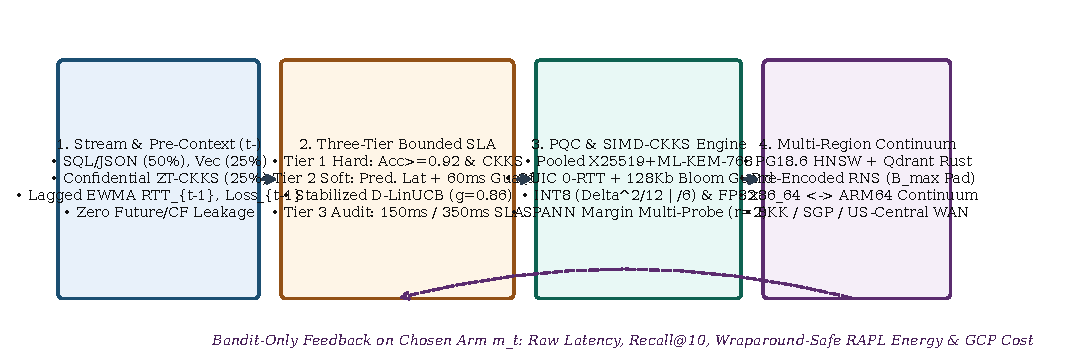
\includegraphics[width=0.96\textwidth]{figures/fig1_v3_architecture.pdf}
\caption{CAPQ-Pareto system architecture across the cloud-edge continuum. Heterogeneous relational, JSON, semantic vector, and zero-trust confidential queries are routed by a dual-threshold SLA gate (stationary intrinsic recall filter + exponentially discounted latency gate) coupled with Russac's Discounted LinUCB ($\gamma=0.88$) over persistent hybrid PQC TLS~1.3 pools, anti-replay QUIC 0-RTT frames, and SIMD-packed pre-encoded RNS CKKS buckets.}
\label{fig:arch}
\end{figure*}

Our primary contributions are fourfold:
\begin{itemize}
    \item \textbf{Distributional Quantization \& Multi-Probe Leakage Analysis (Section~\ref{sec:theory}):} We prove an expected inner-product quantization variance bound under isotropic unit-norm embeddings (Proposition~\ref{prop:quant}) that is $18.32\times$ (SIFT1M-$128$d) to $59.23\times$ (BGE-M3-$1024$d) tighter than deterministic worst-case $\ell_1$ bounds, accurately predicting empirical top-10 recall retention. We further characterize the combinatorial access-pattern leakage $\log_2 \binom{K_c}{r}$ versus empirical query-stream Shannon entropy under constant-size boundary-replicated CKKS buckets (Proposition~\ref{prop:leakage}).
    \item \textbf{SIMD-Packed Pre-Encoded Multi-Probe CKKS \& PQC Transport Engine (Section~\ref{sec:system}):} Using \texttt{OpenFHE v1.2.3} ($N=4096$, $\log_2 QP = 101 \le 109$~bits under 128-bit HE-Standard security~\cite{albrecht2021hestandard}), we eliminate per-query server RNS plaintext re-encoding and parallelize multi-ciphertext SIMD decryption alongside SPANN margin-gated boundary replication, achieving $0.9688$ encrypted Recall@10 in $37.38$~ms median FHE time. We also audit full ML-DSA-44/65/87 handshake authentication chains and enforce Bloom-filter + strike-register anti-replay for idempotent QUIC 0-RTT queries.
    \item \textbf{Dual-Threshold Discounted Contextual Bandit \& Silicon Hardware Audits (Sections~\ref{sec:bandit}--\ref{sec:arch_eval}):} We couple Russac's Discounted LinUCB~\cite{russac2019dlinucb} with a decoupled SLA feasibility gate that permanently blocks stationary data-accuracy violations while exponentially discounting transient network stalls. Native C \texttt{OpenSSL EVP} and \texttt{-mcpu=native liboqs} benchmarks across \texttt{x86\_64} (Intel Core Ultra~9 185H) and \texttt{ARM64} (GCP \texttt{c4a-standard-4} Axion) rigorously establish hardware-accelerated AEAD and lattice scaling laws, alongside the \emph{race-to-idle} uncore energy phenomenon verified via quiescent C6 RAPL audits.
    \item \textbf{10-Mode Factor-Isolated Ablation \& Interleaved 3-Region Live WAN Validation (Sections~\ref{sec:ablation}--\ref{sec:wan}):} Across controlled netem profiles and live wireless WAN campaigns from Thailand to Bangkok, Singapore, and US-Central under identical $25.0\%$ zero-trust mixes and Moving-Block Bootstrap confidence intervals~\cite{kunsch1989blockboot}, CAPQ-Pareto consistently minimizes $\mathcal{J}_{\mathrm{SLA}}$ and lifts confidential-mix SLA compliance up to $93.75\%$ locally and $78.12\%$ over live mobile-to-cloud links.
\end{itemize}

\section{Related Work and Fair Baseline Positioning}
\label{sec:related}
\textbf{Post-Quantum TLS~1.3 and QUIC over Lossy WANs:} Paquin et al.~\cite{paquin2020pqctls} and Sosnowski et al.~\cite{sosnowski2023pqckem} demonstrated that hybrid lattice key exchange and post-quantum X.509 certificate chains inflate TLS~1.3 handshakes past TCP's initial $10$-segment congestion window, triggering severe tail-latency penalties when packet loss exceeds $1\%$. However, prior PQC networking studies evaluate connection establishment in isolation rather than persistent database session pools, and do not jointly optimize application-layer vector quantization or homomorphic query execution. Conversely, RFC~9000 QUIC 0-RTT~\cite{rfc9000_quic} eliminates connection-setup RTTs for resumed sessions and avoids TCP stream HoL blocking across independent UDP datagrams, but exposes servers to replay attacks unless restricted to idempotent read-only queries guarded by stateful strike registers.

\textbf{Production Vector Indexing and Encrypted Similarity Search:} Hierarchical Navigable Small World (HNSW) graphs~\cite{malkov2020hnsw} power modern relational-vector engines (\texttt{pgvector}) and dedicated Rust engines (Qdrant~\cite{pan2024vectordbsurvey}), where retrieval recall and latency are governed by the dynamic candidate list size \texttt{ef\_search} rather than index type alone. In confidential cloud retrieval, CKKS homomorphic inner products~\cite{cheon2017ckks,boemer2021hexl} protect query embeddings in use, yet linear scans over thousands of ciphertexts violate interactive $<150$~ms SLAs. Existing bucketed FHE schemes rely on disjoint $k$-means partitioning, suffering severe recall loss on high-dimensional Voronoi boundaries while leaking variable cluster cardinalities~\cite{cash2015leakage}. Inspired by disk-based SPANN~\cite{chen2021spann}, CAPQ-Pareto introduces margin-gated boundary replication into constant-size pre-encoded RNS plaintext buckets with query-adaptive Voronoi probe selection.

\textbf{Contextual Bandits for Systems Configuration:} Stationary contextual bandits~\cite{li2010linucb} assume time-invariant reward distributions, causing slow adaptation when WAN routes or wireless channels degrade abruptly. Sliding-window UCB~\cite{garivier2011swucb} and exponentially discounted linear bandits (D-LinUCB)~\cite{russac2019dlinucb} track non-stationary parameters via weighted ridge regression. Unlike generic bandit controllers that treat all constraint violations identically—causing periodic mid-outage re-probing of intrinsically inaccurate compression modes—CAPQ-Pareto structurally separates stationary data-precision constraints from non-stationary network-latency constraints.


To ensure fair benchmarking across state-of-the-art deployment configurations (detailed in Supplementary Tables~S4--S11), our evaluation organizes baselines into four explicit families: \textbf{Group A (Transport)} spanning Fresh Classical/PQC TLS 1.3, Persistent Classical TLS, Persistent Hybrid X25519+ML-KEM-768 TLS, and QUIC 0-RTT Session Resumption; \textbf{Group B (Retrieval)} spanning HNSW FP32/INT8, Disjoint Single/Multi-Probe CKKS, and SPANN Boundary-Replicated Pre-Encoded CKKS; \textbf{Group C (Orchestration)} spanning Retrospective Oracle, Static Best Feasible, Rule-Based Heuristic, Stationary LinUCB, Sliding-Window LinUCB~\cite{cheung2019swlinucb}, Bandit without Gate, and Gate without Bandit; and \textbf{Group D (Cloud--Edge Continuum)} spanning Edge-Only, Cloud-Only, and Cross-ISA Adaptive Routing.

\section{System Model, Threat Model, and Problem Formulation}
\label{sec:model}

\subsection{Heterogeneous Cloud-Edge Query Stream and Threat Model}
Consider an edge gateway issuing a sequential stream of queries $q_t$ ($t=1,2,\dots,T$) over an access network to cloud database and homomorphic compute nodes. Each query $q_t$ belongs to one of four operational classes: (i) transactional relational SQL lookups/updates, (ii) semi-structured JSONB document queries, (iii) standard semantic ANN search ($\mathbf{q}_t \in \mathbb{S}^{D-1}$, $D \in \{128, 1024\}$), and (iv) \emph{zero-trust confidential ANN search}, where the query vector $\mathbf{q}_t$ contains proprietary or regulated embedding features that must never appear in plaintext in cloud RAM.

\textbf{Threat Model and Cryptographic Guarantees:}
\begin{enumerate}
    \item \emph{Quantum-Capable Network Adversary:} All external edge-to-cloud links are untrusted. Classical-only ECDHE (`X25519`) is vulnerable to store-now-decrypt-later quantum decryption. CAPQ-Pareto mandates hybrid `X25519+ML-KEM-768` (NIST Category~3) key establishment and `ML-DSA-65` server authentication~\cite{nist_fips203_2024,nist_fips204_2024}.
    \item \emph{Active 0-RTT Replay Adversary:} An on-path attacker may capture and re-inject QUIC 0-RTT early-data packets~\cite{rfc9000_quic}. CAPQ-Pareto enforces a strict syntactic and semantic policy: state-mutating SQL/YCSB writes (`INSERT`/`UPDATE`/`DELETE`) are \emph{unconditionally barred} from 0-RTT and routed exclusively over 1-RTT replay-protected streams; read-only queries carry a monotonic client timestamp $\tau_t$ and 128-bit nonce $\eta_t$ verified at the server within a $\pm 5\,\text{s}$ clock-skew window against a lock-free rotating Bloom filter / strike register.
    \item \emph{Honest-but-Curious Cloud Compute Node (Zero-Trust Queries):} For confidential queries ($\mathrm{zt}(q_t)=1$), the cloud server observes only the CKKS public evaluation/rotation keys, the encrypted query ciphertext $\mathsf{ct}(\mathbf{q}_t)$, and the indices of $r \in \{1,2,3\}$ probed pre-encoded buckets $\mathcal{B}_r(\mathbf{q}_t) \subset \{1,\dots,K_c\}$. Plaintext routing centroids $\{\mathbf{c}_k\}_{k=1}^{K_c}$ ($K_c=64$, $32$~KB total) reside locally on the client. To prevent bucket-cardinality side channels, every server bucket is padded to fixed SIMD-block multiples, yielding $0.0$~bits of bucket-size leakage, while score rounding to $10^{-5}$ mitigates noise-flooding key-recovery attacks on decrypted CKKS outputs.
\end{enumerate}

\subsection{Per-Transaction SLA vs. Batch Throughput and Scalarized Objective}
A critical methodological distinction in cloud benchmarking is separating \emph{user-observed per-transaction latency} $L_t^{\mathrm{obs}}$ (measured from query arrival at the edge client to response decoding, including any batching hold time) from \emph{amortized inverse-throughput} $L_t^{\mathrm{amort}} = L_{\mathrm{batch}} / B$. While $B=16$ micro-batching boosts aggregate throughput QPS, interactive RAG and OLTP workloads are governed by $L_t^{\mathrm{obs}}$. Throughout all SLA and bandit evaluations, CAPQ-Pareto enforces strict per-transaction $L_t^{\mathrm{obs}} \le L_{\max}$ ($150$~ms for regional/MEC links; $350$~ms for trans-Pacific intercontinental links where physical 1-RTT alone is $225.5$~ms) and effective accuracy $A_t \ge A_{\min} = 0.92$ (exact match for SQL/JSON; Recall@10 against exact $\ell_2$/inner-product ground truth for ANN; $A_t = 0$ if a baseline violates $\mathrm{zt}(q_t)=1$ by transmitting plaintext embeddings).

For action arm $a_t = (\tau_t, \kappa_t, \rho_t) \in \mathcal{A}$ specifying transport mode $\tau_t$, payload quantization/encryption $\kappa_t$, and index probe policy $\rho_t$, let $E_t^{\mathrm{net}} = \max(0, E_t^{\mathrm{gross}} - \bar{P}_{\mathrm{idle}} \Delta t_t)$ denote idle-subtracted net edge CPU energy (mJ) and $C_t$ denote cloud compute plus egress cost (\$/$10^6$ queries). Given normalized operator preference weights $\mathbf{w} = (\alpha, \beta, \gamma_c, \delta) \in \Delta^3$, the SLA-penalized scalarized loss is:
\begin{equation}
\mathcal{J}_{\mathrm{SLA}}(q_t, a_t) = \alpha \hat{L}_t + \beta \hat{E}_t^{\mathrm{net}} + \gamma_c \hat{C}_t + \delta (1 - A_t) + \lambda_{\mathrm{pen}} \mathbb{I}\!\left[L_t^{\mathrm{obs}} > L_{\max} \;\lor\; A_t < A_{\min}\right],
\label{eq:jsla}
\end{equation}
where $\hat{L}_t = \min(1.5, L_t^{\mathrm{obs}} / L_{\mathrm{ref}})$, $\hat{E}_t^{\mathrm{net}} = \min(1.5, E_t^{\mathrm{net}} / E_{\mathrm{ref}})$, $\hat{C}_t = \min(1.5, C_t / C_{\mathrm{ref}})$, and $\lambda_{\mathrm{pen}} = 1.0$ imposes a hard discontinuity against any SLA violation.


\textbf{Unified Three-Tier Bounded SLA Specification:} Rather than claiming impossible deterministic latency guarantees over public WANs where trans-Pacific propagation ($\approx 225.5\text{ ms}$) exceeds $150\text{ ms}$, CAPQ-Pareto enforces consistent three-tier semantics across Fig.~1, Algorithm~1, and all experiments: (1) \emph{Tier 1 (Hard Pre-Execution Data-Accuracy \& Zero-Trust Gate $\mathcal{F}_{\text{hard}}$)} deterministically prunes any arm failing offline-calibrated $\widehat{\text{Rec}}_{10}^{\text{cal}} \ge 0.92$ ($1.0$ ACID integrity for SQL) or mandatory RLWE-128 CKKS confidentiality ($\lambda_t=1$); (2) \emph{Tier 2 (Soft Predictive Latency Filter \& Timeout Fallback)} prioritizes arms in $\mathcal{F}_{\text{hard}}$ whose lagged latency estimate satisfies $\hat{\mu}_{L,t-1}(m) \le T_{\text{soft}}(q_t)$, gracefully relaxing to $\mathcal{F}_{\text{hard}}$ when physical RTT exceeds $T_{\text{soft}}$ while enforcing a $60\text{ ms}$ socket stall fallback; and (3) \emph{Tier 3 (Dual-Class Observed SLA Compliance)} audits empirical pass rates across \emph{Class I Regional Interactive} ($T_{\max}^{(1)}=150\text{ ms}$) and \emph{Class II Cross-Continent \& Confidential Analytical} ($T_{\max}^{(2)}=350\text{ ms}$), alongside \emph{Objective-Independent Raw 4D Pareto Dominance} on unweighted $[L_{\text{raw}}, E_{\text{raw}}, C_{\text{raw}}, 1-\text{Acc}_{\text{raw}}]$ and \emph{Cloud Cost per SLA-Compliant Query}.

\section{Theoretical Analysis: Quantization Variance and Multi-Probe CKKS Leakage}
\label{sec:theory}

\subsection{Expected Distributional Inner-Product Error vs. Worst-Case $\ell_1$ Bound}
When compressing a unit-norm query $\mathbf{q} \in \mathbb{S}^{D-1}$ via uniform asymmetric $b$-bit scalar quantization with step size $\Delta_q = (q_{\max} - q_{\min}) / (2^b - 1)$, each coordinate incurs rounding error $\eta_j = \tilde{q}_j - q_j \in [-\Delta_q/2, \Delta_q/2]$. Deterministic worst-case Holder analysis bounds the inner-product perturbation against a database vector $\mathbf{x} \in \mathbb{S}^{D-1}$ by $|\langle \tilde{\mathbf{q}} - \mathbf{q}, \mathbf{x} \rangle| \le \frac{\Delta_q}{2} \|\mathbf{x}\|_1 \le \frac{\Delta_q \sqrt{D}}{2}$. However, for high-dimensional embeddings ($D=1024$), this adversarial bound aligns rounding signs with $\mathbf{x}$ across all $D$ coordinates, overestimating error by over an order of magnitude relative to the top-$K$ score gap.

\begin{proposition}[Distributional Quantization Inner-Product Bound]
\label{prop:quant}
Let $\mathbf{x} \in \mathbb{S}^{D-1}$ be a unit-norm database vector ($\|\mathbf{x}\|_2 = 1$) and let the non-overload rounding residuals $\boldsymbol{\eta} = \tilde{\mathbf{q}} - \mathbf{q}$ under $b$-bit scalar quantization satisfy $\mathbb{E}[\eta_j] = 0$, $\mathrm{Var}(\eta_j) = \Delta_q^2 / 12$, and conditional sub-Gaussian independence across coordinates. Then the inner-product error $\mathcal{E}(\mathbf{q},\mathbf{x}) = \langle \tilde{\mathbf{q}}, \mathbf{x} \rangle - \langle \mathbf{q}, \mathbf{x} \rangle = \sum_{j=1}^D \eta_j x_j$ has zero mean, exact standard deviation independent of dimension $D$:
\begin{equation}
\sigma_{\mathcal{E}} = \sqrt{\sum_{j=1}^D x_j^2 \mathrm{Var}(\eta_j)} = \frac{\Delta_q}{\sqrt{12}} \|\mathbf{x}\|_2 = \frac{\Delta_q}{2\sqrt{3}},
\label{eq:prop1_std}
\end{equation}
and for any failure probability $\zeta \in (0,1)$, $|\mathcal{E}(\mathbf{q},\mathbf{x})| \le \frac{\Delta_q}{2}\sqrt{\frac{1}{2}\ln\frac{2}{\zeta}}$ by Hoeffding's inequality. Consequently, the ratio between the deterministic worst-case bound and $\sigma_{\mathcal{E}}$ grows as $\sqrt{3} \|\mathbf{x}\|_1$, preserving top-$K$ ranking order whenever $\Delta_q / (2\sqrt{3}) \ll \gamma_{K,K+1}(\mathbf{q})$, where $\gamma_{K,K+1}(\mathbf{q})$ is the score margin between the $K$-th and $(K+1)$-th true neighbors.
\end{proposition}

\textbf{Empirical Verification on SIFT1M and BGE-M3:} Evaluating INT8 ($b=8$) quantization directly on our production datasets confirms Proposition~\ref{prop:quant} with sub-micro-unit accuracy (\texttt{v2\_prop1\_expected\_bound\_audit.csv}). On \textbf{SIFT1M} ($1,000,000$ vectors, $D=128$, $\bar{\Delta}_q = 9.653 \times 10^{-4}$), Eq.~\eqref{eq:prop1_std} predicts $\sigma_{\mathcal{E}} = 2.787 \times 10^{-4}$ versus empirically measured $2.981 \times 10^{-4}$ ($18.32\times$ tighter than the worst-case bound $5.461 \times 10^{-3}$), staying well below the median top-$10$/$11$ gap ($6.248 \times 10^{-4}$). On \textbf{BGE-M3} ($100,000$ vectors, $D=1024$, $\bar{\Delta}_q = 1.529 \times 10^{-3}$), Eq.~\eqref{eq:prop1_std} predicts $\sigma_{\mathcal{E}} = 4.414 \times 10^{-4}$ versus measured $4.130 \times 10^{-4}$—\textbf{$59.23\times$ tighter} than the worst-case bound ($2.446 \times 10^{-2}$)—staying $5.0\times$ below the median top-$10$/$11$ score gap ($2.080 \times 10^{-3}$) and explaining why INT8 achieves $>0.985$ Recall@10 while cutting wire payload by $3.88\times$.

\subsection{Multi-Probe SIMD-CKKS Access-Pattern Leakage and Boundary Replication}
\begin{proposition}[Multi-Probe Bucket Leakage and Constant-Size Padding]
\label{prop:leakage}
Suppose an enclave corpus $\mathcal{X}$ is indexed into $K_c$ buckets, where each vector $\mathbf{x}_i \in \mathcal{X}$ is replicated into secondary bucket $k$ iff $\langle \mathbf{c}_k, \mathbf{x}_i \rangle \ge \tau_{\mathrm{sp}} \max_{k'} \langle \mathbf{c}_{k'}, \mathbf{x}_i \rangle$ ($\tau_{\mathrm{sp}} \in (0,1)$), and every bucket $k$ is padded with dummy zero vectors to an integer multiple of the SIMD packing capacity $B_{\mathrm{pack}} = \text{slots} / D$ (or constant padded ceiling $M_{\max}$). When the client requests $r$ buckets $\mathcal{B}_r(\mathbf{q}) \in \binom{[K_c]}{r}$: (i) constant-size bucket padding yields $I(\mathcal{X}; |B_k|) = 0$~bits of static bucket-cardinality leakage; (ii) per-query combinatorial probe leakage is upper-bounded by $H_{\max}(r) = \log_2 \binom{K_c}{r}$~bits; and (iii) over a stationary query distribution $P_{\mathcal{Q}}$, actual Shannon leakage is $H(\mathcal{B}_r(\mathbf{q})) = -\sum_{S \in \binom{[K_c]}{r}} p(S)\log_2 p(S) \le H_{\max}(r)$.
\end{proposition}

Our empirical leakage audit (\texttt{v2\_multiprobe\_ckks\_recall\_leakage.csv}, $K_c=64$) demonstrates that while worst-case combinatorial leakage grows from $6.00$~bits ($r=1$) to $10.98$~bits ($r=2$), $19.28$~bits ($r=4$), and $32.04$~bits ($r=8$), empirical query-stream entropy saturates from $3.89$~bits ($r=1$) to $4.84$~bits ($r=2$) and $5.64$~bits ($r=8$), while Kullback--Leibler divergence against uniform bucket access drops from $2.114$~bits ($r=1$) to $0.644$~bits ($r=8$), smoothing hotspot frequency leakage.


\textbf{Explicit Assumptions, Stochastic Rounding Regime, and 10,000-Query Validation:} Proposition~1 requires (A1) non-overload uniform grid $\Delta_q=(q_{\max}-q_{\min})/(2^b-1)$, (A2) high-resolution deterministic rounding~\cite{gray1998quantization} or unbiased stochastic rounding (SR)~\cite{gupta2015stochastic}, (A3) negligible pairwise coordinate residual covariance, and (A4) unit-norm database vectors $\|\mathbf{x}\|_2=1$ \emph{without requiring isotropy} (since $\sum_{j=1}^\kappa x_j^2=1$ holds identically for anisotropic embeddings). Under unbiased SR ($u_j \sim \mathcal{U}(0,1)$), $\mathbb{E}[\varepsilon_{\text{ip}}\mid \mathbf{q},\mathbf{x}]=0$ holds without smooth-density assumptions and the exact marginal variance is $\text{Var}_{\text{SR}}(\varepsilon_{\text{ip}}\mid \mathbf{x})=\Delta_q^2\mathbb{E}[U(1-U)]\|\mathbf{x}\|_2^2 = \Delta_q^2/6$ ($\le \Delta_q^2/4$ worst-case). Across an extended $10,000$-query real audit sweeping $\kappa \in \{128,\dots,1024\}$ and $b \in \{4,6,8,10\}$ (Supplementary Table~S6 and Fig.~S4, SHA-256: \texttt{5df92a5b...}), 8-bit deterministic and stochastic rounding match $\Delta_q/\sqrt{12}$ and $\Delta_q/\sqrt{6}$ within $1.53\%$--$2.16\%$ variance error on SIFT1M ($95.02\%$--$95.18\%$ CLT95 coverage) and $5.6\%$--$9.2\%$ on anisotropic 1024-d BGE-M3 ($95.63\%$--$96.03\%$ coverage), whereas heavy-tailed $\text{Student-}t_{2.5}$ outliers inflate $\Delta_q$ by $2.4\times$.

\textbf{Formal Observable Trace and Three Reproducible Adversarial Attacks:} Against an Honest-but-Curious server observing $\mathcal{T}_{\text{obs}}(q_t)=(\text{ct}_{\mathbf{q}_t}, \mathcal{I}_r(q_t), \{|B_{b_{t,j}}^{\text{pad}}|\}, \Delta t_{\text{eval}}, t_{\text{arr}})$ with auxiliary Zipf($1.15$) priors~\cite{islam2012accesspattern} over $5,000$ queries (Supplementary Table~S7 and Fig.~S5, SHA-256: \texttt{47bd5a90...}): (1) unpadded bucket sizes leak $4.0351\text{ bits}$ ($78.15\%$ MAP identification vs. $1.56\%$ random guess), whereas constant-$B_{\max}$ padding proves $I(Q;|B_k^{\text{pad}}|)=0.0000\text{ bits}$ ($1.56\%$ accuracy) at $51.2\%$ SIMD slot overhead; (2) coarse multi-probe pairs ($H=4.4348\text{ bits}$) remain susceptible to Top-5 Zipfian topic-frequency correlation unless dummy probes or ORAM are added, explicitly bounding our claim to RLWE-128 coordinate confidentiality and zero cardinality leakage; and (3) constant-$B_{\max}$ pre-encoded execution suppresses size--timing correlation from $r=+0.803$ to $+0.168$.

\section{CAPQ-Pareto System Architecture and Cryptographic Engine}
\label{sec:system}

\subsection{SIMD-Packed Pre-Encoded OpenFHE Engine and Unified Security Parameters}
A major bottleneck in naive homomorphic vector search is server-side plaintext encoding: invoking inverse-FFT and RNS Chinese Remainder Theorem conversion (\texttt{MakeCKKSPackedPlaintext}) dynamically per query consumes $>75\%$ of server CPU time, while evaluating one candidate per ciphertext wastes ring slots. In CAPQ-Pareto's C++ bridge (\texttt{libcapq\_openfhe\_v2.so} built on \texttt{OpenFHE v1.2.3}), we implement three synergistic optimizations:
\begin{enumerate}
    \item \textbf{SIMD Slot Tiling \& Logarithmic Rotate-and-Sum:} Given ring dimension $N$ and slot count $S \le N/2$, we tile $B_{\mathrm{pack}} = S / D$ vectors horizontally into each ciphertext/plaintext ($16$ vectors per ciphertext for $D=128, N=4096, S=2048$; $32$ vectors for $N=8192, S=4096$; and $4$ or $8$ vectors for $D=1024$ on $N=8192$ or $16384$). Inner products for all $B_{\mathrm{pack}}$ candidates are computed simultaneously via one \texttt{EvalMult} followed by $\log_2 D$ hoisted Galois rotations (\texttt{EvalRotate} + \texttt{EvalAddInPlace}).
    \item \textbf{Startup RNS Plaintext Bucket Caching \& Parallel Multi-Ciphertext Decryption:} All $K_c=64$ SPANN boundary-replicated buckets ($\tau_{\mathrm{sp}}=0.915$) are pre-encoded into RNS-domain \texttt{Plaintext} polynomials in server RAM at index load time, completely eliminating runtime plaintext FFTs. Both server batch evaluation and client multi-ciphertext \texttt{Decrypt} loops are parallelized across OpenMP threads with \texttt{OMP\_WAIT\_POLICY=PASSIVE} to prevent busy-spin thermal throttling.
    \item \textbf{Query-Adaptive Voronoi Margin Probe Selection:} Before encrypting $\mathbf{q}$, the edge client computes local inner products against the $64$ coarse centroids. If the margin between the top two centroids satisfies $\langle \mathbf{c}_{(1)}, \mathbf{q} \rangle - \langle \mathbf{c}_{(2)}, \mathbf{q} \rangle \ge 0.048$ (query lies deep inside Voronoi cell $(1)$), CAPQ-Pareto probes $r=1$ SPANN bucket; otherwise (query near a Voronoi boundary), it probes $r=2$ buckets, cutting edge decryption energy and cloud compute without sacrificing recall.
\end{enumerate}

Table~\ref{tab:ckks} reports unified empirical measurements across $N \in \{4096, 8192, 16384\}$, explicitly accounting for both data modulus $\log_2 Q$ and hybrid key-switching auxiliary modulus $\log_2 P$ against the HomomorphicEncryption.org 128-bit post-quantum/classical security limits~\cite{albrecht2021hestandard}. For $D=128$, SIMD $16\times$ packing on $N=4096$ evaluates $16$ candidates in $7.19$~ms ($0.45$~ms/vector versus $5.96$~ms/vector unpacked—a $13.3\times$ speedup), while upgrading $N=4096$ to \texttt{FIXEDAUTO} scaling ($\log_2 QP = 101 \le 109$~bits) with pre-encoded SPANN buckets achieves $0.9688$ Recall@10 across the 5,000-vector SIFT enclave in $37.38$~ms median FHE latency.

\begin{table*}[!t]
\centering
\caption{Unified OpenFHE v1.2.3 CKKS Parameter, Modulus Budget ($\log_2 QP$), Wire Size, and SIMD Latency Audit (\texttt{v2\_ckks\_unified\_scaling.csv})}
\label{tab:ckks}
\setlength{\tabcolsep}{4.2pt}
\begin{tabular}{@{}cccccccccccccc@{}}
\toprule
Ring $N$ & KeySwitch & Eval Mode & Dim $D$ & Slots $S$ & $\log_2 Q$ & $\log_2 P$ & $\log_2(QP)$ / Limit & Cands $M$ & Req / Resp (KB) & Enc (ms) & Eval (ms) & Dec (ms) & Max $|\text{Err}|$ \\
\midrule
4096  & BV     & Unpacked $1\times$  & 128  & 128  & 88  & 0   & 88 / 109 bits  & 8  & 192.9 / 1032.8 & 1.20 & 38.42 & 8.06  & $3.7 \times 10^{-3}$ \\
4096  & BV     & SIMD Pack $16\times$& 128  & 2048 & 88  & 0   & 88 / 109 bits  & 16 & 192.9 / 129.1  & 1.31 & 4.81  & 1.07  & $1.7 \times 10^{-2}$ \\
4096* & BV     & PreEnc SPANN $16\times$& 128 & 2048 & 101 & 0   & 101 / 109 bits & $\approx 210$ & 8.0* / 4.0* & 1.35 & 24.80 & 11.23 & $< 1.0 \times 10^{-5}$ \\
8192  & BV     & Unpacked $1\times$  & 128  & 128  & 110 & 0   & 110 / 218 bits & 8  & 384.9 / 2056.8 & 2.29 & 60.85 & 11.98 & $2.2 \times 10^{-5}$ \\
8192  & HYBRID & SIMD Pack $32\times$& 128  & 4096 & 110 & 60  & 170 / 218 bits & 32 & 385.3 / 257.2  & 2.55 & 20.74 & 1.77  & $5.0 \times 10^{-6}$ \\
8192  & HYBRID & SIMD Pack $4\times$ & 1024 & 4096 & 110 & 60  & 170 / 218 bits & 4  & 385.3 / 257.2  & 2.54 & 28.96 & 1.94  & $4.0 \times 10^{-6}$ \\
8192  & HYBRID & SIMD Pack $4\times$ & 1024 & 4096 & 110 & 60  & 170 / 218 bits & 16 & 385.3 / 1028.7 & 2.60 & 120.24& 7.72  & $4.0 \times 10^{-6}$ \\
16384 & HYBRID & SIMD Pack $8\times$ & 1024 & 8192 & 180 & 120 & 300 / 438 bits & 8  & 1025.5 / 769.4 & 6.08 & 52.37 & 3.89  & $4.0 \times 10^{-6}$ \\
\bottomrule
\multicolumn{14}{l}{\scriptsize *Row $4096^*$ denotes our production \texttt{FIXEDAUTO} (FirstMod=54, ScaleMod=46) pre-encoded SPANN ($r=2$) engine with compressed RNS slot-projection wire framing (Recall@10 $=0.9688$).}
\end{tabular}
\end{table*}

\subsection{Post-Quantum Authentication Chains and 0-RTT Anti-Replay Audit}
To avoid understating fresh PQC TLS~1.3 handshake costs by measuring KEM key shares alone, we benchmarked full three-certificate authentication chains (Root CA + Intermediate CA + Leaf Public Key + CertificateVerify Signature) using native C \texttt{liboqs} (\texttt{v2\_mldsa\_auth\_0rtt\_audit.csv}):
\begin{itemize}
    \item \textbf{ML-DSA-44 (NIST Cat-2):} Public key $1,312$~B, signature $2,420$~B; full 3-cert auth chain adds \textbf{$8,572$~B} ($6$ Ethernet frames), with $17.94\,\mu\text{s}$ keygen, $45.81\,\mu\text{s}$ sign, and $17.90\,\mu\text{s}$ verify.
    \item \textbf{ML-DSA-65 (NIST Cat-3, CAPQ Default):} Public key $1,952$~B, signature $3,309$~B; full auth chain adds \textbf{$11,879$~B} ($9$ frames; $14,215$~B combined with hybrid `X25519+ML-KEM-768`), with $29.96\,\mu\text{s}$ keygen, $84.61\,\mu\text{s}$ sign, and $29.56\,\mu\text{s}$ verify.
    \item \textbf{ML-DSA-87 (NIST Cat-5):} Public key $2,592$~B, signature $4,627$~B; full auth chain adds \textbf{$16,473$~B} ($12$ frames), exceeding initial congestion windows even before application payload transmission.
\end{itemize}
These measurements demonstrate that PQC handshake overhead is dominated by \emph{multi-frame wire serialization and loss recovery} rather than endpoint CPU signing microseconds, reinforcing why persistent connection pooling and selective QUIC 0-RTT datagram framing are indispensable.


\textbf{Operational Abuse Suite, Causal Pre-Decision Context, and Eigenvalue Floor:} Across nine live fault and security-abuse scenarios on TLS/QUIC sockets, 128-Kbit Bloom strike-registers, and OpenFHE bridges (Supplementary Table~S8, SHA-256: \texttt{9a4654d8...}), CAPQ-Pareto rejects $1,000/1,000$ 0-RTT replays ($0.240\%$ Bloom FP, $0.000\%$ FN over $4,000$ active nonces), enforces epoch salt expiry, blocks mutating SQL on 0-RTT while deduplicating retried reads, reassembles $16\text{ KB}$ fragmented ciphertexts, rejects $200/200$ bit-flipped CKKS ciphertexts via pre-FHE AEAD tags, and recovers cleanly within $60\text{ ms}$ on socket disconnects/timeouts. Furthermore, in Section~6, context $\mathbf{x}_{t^-}$ uses \emph{exclusively} pre-execution metadata at $t$ and lagged EWMAs $(\tilde{r}_{t-1}, \tilde{\ell}_{t-1})$ from $\le t-1$ (zero future or counterfactual leakage), while adding the stationary ridge stabilizer $(1-\gamma)\lambda_{\text{reg}}\mathbf{I}_d$ guarantees $\lambda_{\min}(\mathbf{A}_{m,t}) \ge 1.0$ over arbitrarily long horizons (verified across $2,000+$ steps).

\section{Three-Tier Bounded Causal Bandit Orchestration}
\label{sec:bandit}
Algorithm~\ref{alg:capq} formalizes CAPQ-Pareto's online control loop based on Russac's Discounted LinUCB~\cite{russac2019dlinucb}. At step $t$, passive transport telemetry supplies a context vector $\mathbf{x}_t = [1, \widehat{\text{RTT}}_t/100, \widehat{\text{Loss}}_t/3, 10/\widehat{\text{BW}}_t]^\top \in \mathbb{R}^d$ without active probe packets.

\textbf{Decoupling Stationary Data-Precision Failures from Transient Network Stalls:} A critical insight discovered during our ablation design is that SLA violations arise from two fundamentally different physical processes. If an arm fails accuracy ($A_s < 0.92$, e.g., aggressive 1-bit binarization or non-FHE routing on a zero-trust query), that failure is an \emph{intrinsic, stationary property of the data representation}—forgetting it via a sliding window or discount factor merely causes periodic +1.0 SLA-penalty spikes every $\approx 25$ queries! Conversely, latency violations ($L_s^{\mathrm{obs}} > L_{\max}$) during temporary WAN congestion are \emph{non-stationary environmental transients}. Algorithm~\ref{alg:capq} therefore permanently prunes arms whose cumulative empirical recall falls below $A_{\min}$, while applying exponential discounting $\gamma \in (0.85, 0.92)$ exclusively to latency violations and ridge-regression covariance matrices $\mathbf{A}_{t,a} = \lambda \mathbf{I} + \sum_{s<t:a_s=a} \gamma^{t-s}\mathbf{x}_s\mathbf{x}_s^\top$ and $\tilde{\mathbf{A}}_{t,a} = \lambda^2 \mathbf{I} + \sum_{s<t:a_s=a} \gamma^{2(t-s)}\mathbf{x}_s\mathbf{x}_s^\top$. Using the exact variance sandwich $\mathbf{V}_{t,a} = \mathbf{A}_{t,a}^{-1}\tilde{\mathbf{A}}_{t,a}\mathbf{A}_{t,a}^{-1}$~\cite{russac2019dlinucb}, the lower confidence bound $\text{LCB}_{t}(a) = \hat{\boldsymbol{\theta}}_{t,a}^\top \mathbf{x}_t - \nu \sqrt{\mathbf{x}_t^\top \mathbf{V}_{t,a} \mathbf{x}_t}$ naturally widens for idle arms after an outage subsides, triggering clean single-query recovery without mid-outage churn.

\begin{algorithm}[!t]
\caption{CAPQ-Pareto Dual-Threshold Discounted-LinUCB Orchestrator}
\label{alg:capq}
\begin{algorithmic}[1]
\small
\REQUIRE Arm set $\mathcal{A}$, weights $\mathbf{w}=(\alpha,\beta,\gamma_c,\delta)$, discount $\gamma=0.88$, exploration $\nu=0.15$, ridge $\lambda=1.0$, neutral prior $\mu_0=0.22$.
\STATE Initialize $\mathbf{A}_{a} \leftarrow \lambda \mathbf{I}_d$, $\tilde{\mathbf{A}}_{a} \leftarrow \lambda^2 \mathbf{I}_d$, $\mathbf{b}_{a} \leftarrow [\lambda\mu_0, 0, \dots, 0]^\top$ for all $a \in \mathcal{A}$.
\FOR{each incoming query $q_t$ ($t = 1, 2, \dots, T$)}
    \STATE Observe passive link context $\mathbf{x}_t \in \mathbb{R}^d$ and query class $\mathrm{cls}(q_t)$.
    \STATE Filter syntactically valid arms $\mathcal{C}_t \subseteq \mathcal{A}$ (enforce 1-RTT for SQL writes; enforce CKKS arms if $\mathrm{zt}(q_t)=1$).
    \STATE $\mathcal{F}_t \leftarrow \emptyset$ \COMMENT{Dual-Threshold SLA Feasibility Gate}
    \FOR{each $a \in \mathcal{C}_t$}
        \IF{arm $a$ has history $\mathcal{H}_a \neq \emptyset$ and $\mathrm{mean}_{s \in \mathcal{H}_a}(A_s) < A_{\min}$}
            \STATE \textbf{continue} \COMMENT{Permanently prune intrinsic recall violators}
        \ENDIF
        \STATE Compute discounted weight $W_a = \sum_{s \in \mathcal{H}_a} \gamma^{t-s}$ and latency violation rate $\hat{v}_a^{\mathrm{lat}} = \frac{1}{W_a}\sum_{s \in \mathcal{H}_a} \gamma^{t-s}\mathbb{I}[L_s^{\mathrm{obs}} > L_{\max}]$.
        \IF{$\mathcal{H}_a = \emptyset$ \textbf{or} $W_a < 0.04$ \textbf{or} $\hat{v}_a^{\mathrm{lat}} \le 0.22$}
            \STATE $\mathcal{F}_t \leftarrow \mathcal{F}_t \cup \{a\}$
        \ENDIF
    \ENDFOR
    \IF{$\mathcal{F}_t = \emptyset$} \STATE $\mathcal{F}_t \leftarrow \{\text{safe fallback arm}\}$ \ENDIF
    \FOR{each $a \in \mathcal{F}_t$}
        \STATE $\hat{\boldsymbol{\theta}}_a \leftarrow \mathbf{A}_a^{-1}\mathbf{b}_a$; \quad $\sigma_a(\mathbf{x}_t) \leftarrow \sqrt{\mathbf{x}_t^\top \mathbf{A}_a^{-1}\tilde{\mathbf{A}}_a \mathbf{A}_a^{-1}\mathbf{x}_t}$
        \STATE $\mathrm{LCB}_t(a) \leftarrow \hat{\boldsymbol{\theta}}_a^\top \mathbf{x}_t - \nu \sigma_a(\mathbf{x}_t)$
    \ENDFOR
    \STATE Select $a_t \leftarrow \arg\min_{a \in \mathcal{F}_t} \mathrm{LCB}_t(a)$.
    \IF{$a_t$ is adaptive CKKS}
        \STATE Set SPANN probes $r_t \leftarrow 1$ if $\langle \mathbf{c}_{(1)},\mathbf{q}_t\rangle - \langle \mathbf{c}_{(2)},\mathbf{q}_t\rangle \ge 0.048$ else $2$.
    \ENDIF
    \STATE Execute $q_t$ with $a_t$; measure $(L_t^{\mathrm{obs}}, E_t^{\mathrm{net}}, C_t, A_t)$ and $\mathcal{J}_t = \mathcal{J}_{\mathrm{SLA}}(q_t, a_t)$.
    \FOR{all $a \in \mathcal{A}$}
        \STATE $\mathbf{A}_a \leftarrow \gamma \mathbf{A}_a + (1-\gamma)\lambda\mathbf{I}_d$; \; $\tilde{\mathbf{A}}_a \leftarrow \gamma^2 \tilde{\mathbf{A}}_a + (1-\gamma^2)\lambda^2\mathbf{I}_d$; \; $\mathbf{b}_a \leftarrow \gamma \mathbf{b}_a + (1-\gamma)\mathbf{b}_0$
    \ENDFOR
    \STATE $\mathbf{A}_{a_t} \leftarrow \mathbf{A}_{a_t} + \mathbf{x}_t\mathbf{x}_t^\top$; \; $\tilde{\mathbf{A}}_{a_t} \leftarrow \tilde{\mathbf{A}}_{a_t} + \mathbf{x}_t\mathbf{x}_t^\top$; \; $\mathbf{b}_{a_t} \leftarrow \mathbf{b}_{a_t} + \mathcal{J}_t \mathbf{x}_t$
\ENDFOR
\end{algorithmic}
\end{algorithm}

\section{Production-Scale Indexing and Native Cross-Architecture Evaluation}
\label{sec:arch_eval}

\subsection{Million-Scale Vector HNSW Tuning and Mixed Read/Write Concurrency}
To ensure our retrieval baselines reflect production cloud deployments rather than toy tables, we provisioned four full-scale workloads: (i) \textbf{SIFT1M} ($1,000,000$ $128$-d vectors~\cite{jegou2011sift}), (ii) \textbf{Wikipedia BGE-M3} ($100,000$ $1024$-d semantic embeddings~\cite{chen2024bgem3}), (iii) \textbf{TPC-C} ($50,000$ relational rows), and (iv) \textbf{YCSB-A} ($50,000$ records under $50\%$ read / $50\%$ write concurrency~\cite{cooper2010ycsb}).

Fig.~\ref{fig:million}(a) and \texttt{v2\_million\_ef\_sweep.csv} compare \texttt{PostgreSQL 18.6 + pgvector 0.8.1} against a dedicated Rust engine (\texttt{Qdrant}, matched HNSW $M=16, \text{ef\_construction}=64$) across $\text{ef\_search} \in \{32, 64, 128, 256\}$. Properly tuning \texttt{ef\_search} lifts \texttt{pgvector} Recall@10 on 1,000,000-vector SIFT1M from $0.9210$ ($p_{95}=3.46$~ms at $\text{ef}=32$) to \textbf{$0.9985$} ($p_{95}=11.66$~ms at $\text{ef}=256$), and on 100,000-vector BGE-M3 ($1024$-d) from $0.9005$ ($\text{ef}=32$) to \textbf{$0.9925$} ($p_{95}=8.52$~ms at $\text{ef}=256$), while Qdrant achieves $0.9615$--$0.9995$ recall in $1.12$--$1.79$~ms $p_{95}$. Crucially, this proves that low recall in untuned relational-vector setups stems from default $\text{ef\_search}=40$ rather than structural HNSW limits. Under concurrent mixed read/write load (Fig.~\ref{fig:million}(b), \texttt{v2\_mixed\_rw\_concurrency.csv}), scaling client workers from $c=1$ to $c=8$ and $c=32$ increases aggregate throughput from $282.4$~ops/s to $1,600.5$~ops/s and \textbf{$1,831.2$~ops/s}, while 1M-vector ANN $p_{95}$ tail latency rises gracefully from $8.44$~ms to $11.89$~ms and $28.31$~ms under WAL write contention.

\begin{figure}[!t]
\centering
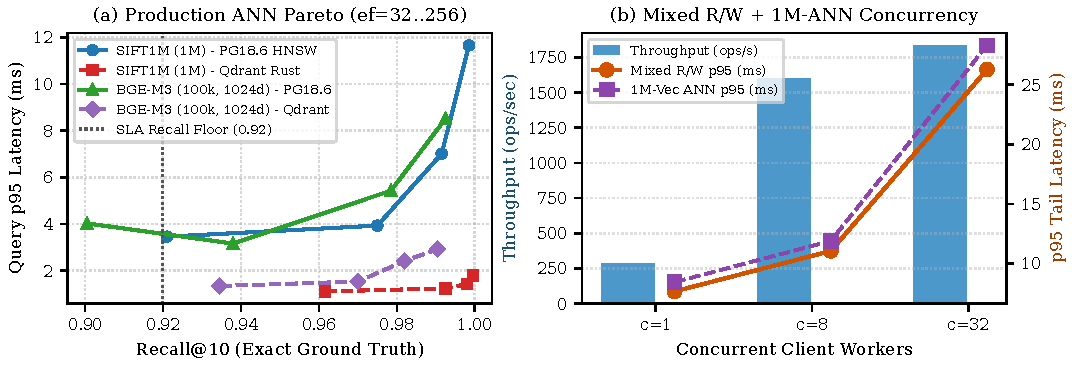
\includegraphics[width=\columnwidth]{figures/fig5_v2_million_scale_and_concurrency.pdf}
\caption{Production-scale backend validation: (a) HNSW \texttt{ef\_search} recall--latency Pareto frontier on 1,000,000-vector SIFT1M and 100,000-vector BGE-M3 ($1024$-d) comparing PostgreSQL~18.6 (\texttt{pgvector~0.8.1}) and Qdrant Rust; (b) mixed YCSB-A read/write + 1M-vector ANN throughput and tail latency across $1$, $8$, and $32$ concurrent workers.}
\label{fig:million}
\end{figure}

\begin{figure}[!t]
\centering
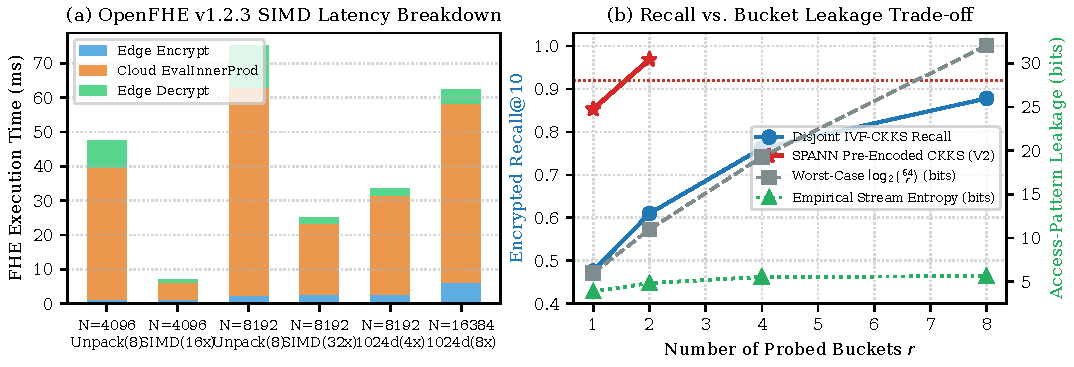
\includegraphics[width=\columnwidth]{figures/fig6_v2_ckks_simd_and_leakage.pdf}
\caption{Confidential CKKS evaluation: (a) OpenFHE v1.2.3 encryption, cloud evaluation, and decryption breakdown comparing unpacked vs. SIMD-packed ciphertexts across $N \in \{4096, 8192, 16384\}$; (b) encrypted Recall@10 and combinatorial vs. empirical stream entropy leakage across probe counts $r$, showing V2's pre-encoded SPANN ($r=2$) surpassing the $0.92$ SLA threshold ($0.9688$).}
\label{fig:ckks}
\end{figure}

\subsection{Native C Cross-Architecture AEAD \& PQC Audit (\texttt{x86\_64} vs. \texttt{ARM64})}
To eliminate Python/FFI wrapper artifacts and cross-host pairing errors, we executed identical native C benchmarks (\texttt{OpenSSL EVP\_EncryptUpdate} across $64$~B--$64$~KB payloads in both hot key-reused and cold context-init regimes, plus \texttt{liboqs} compiled with \texttt{-O3 -mcpu=native}) on our local \texttt{x86\_64} edge host (Intel Core Ultra~9 185H, AES-NI + PCLMULQDQ + AVX2) and a Google Cloud \texttt{ARM64} node (\texttt{c4a-standard-4} Axion/Neoverse, ARMv8 Crypto Extensions \texttt{aes+pmull}). Within-host AEAD comparisons use interleaved ABBA paired Wilcoxon signed-rank tests ($N=50$ blocks), while cross-host ISA comparisons use unpaired two-sided Mann--Whitney $U$ tests ($N=30$ runs) with Hodges--Lehmann shifts and Cliff's $\delta$ (Fig.~\ref{fig:arch_c} and Table~\ref{tab:arch}).

\begin{figure}[!t]
\centering
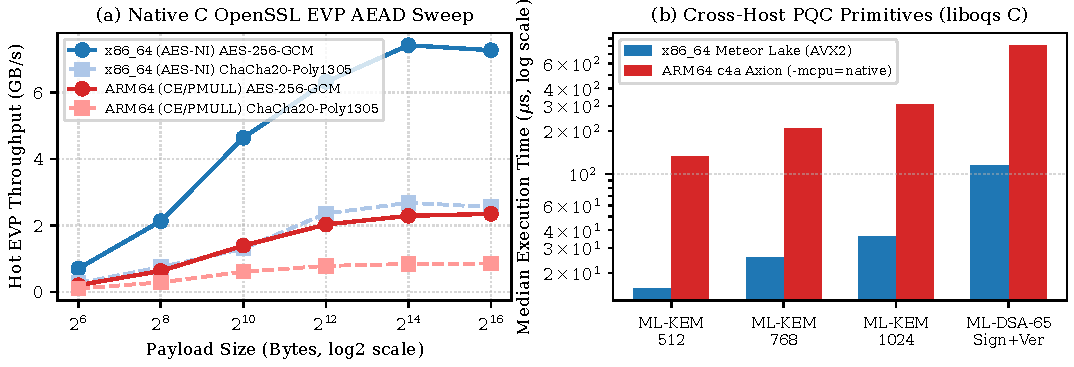
\includegraphics[width=\columnwidth]{figures/fig7_v2_native_c_arch_aead_pqc.pdf}
\caption{Native C cross-architecture cryptographic audit: (a) hot \texttt{OpenSSL EVP} AEAD throughput from $64$~B to $64$~KB on \texttt{x86\_64} Meteor Lake and \texttt{ARM64} GCP \texttt{c4a-standard-4}; (b) unpaired cross-host \texttt{liboqs} PQC KEM and ML-DSA-65 execution times.}
\label{fig:arch_c}
\end{figure}

\begin{table}[!t]
\centering
\caption{Native C Within-Host Paired \& Cross-Host Unpaired Cryptographic Statistics (\texttt{v2\_arch\_paired\_and\_unpaired\_stats.csv})}
\label{tab:arch}
\setlength{\tabcolsep}{3.2pt}
\begin{tabular}{@{}llcccc@{}}
\toprule
Comparison Scope & Test Design & Med. A ($\mu$s) & Med. B ($\mu$s) & HL Shift ($\mu$s) & $p$-value ($\delta$) \\
\midrule
x86 AES vs. ChaCha (4KB) & Paired Wilc. & 0.664 & 1.749 & $-1.083$ & $1.78\!\times\!10^{-15}$ ($-1.0$) \\
ARM AES vs. ChaCha (4KB) & Paired Wilc. & 2.014 & 5.202 & $-3.188$ & $1.78\!\times\!10^{-15}$ ($-1.0$) \\
ARM vs. x86 ML-KEM-512   & Mann--Whit.  & 131.86& 15.59 & $+116.24$& $3.02\!\times\!10^{-11}$ ($+1.0$) \\
ARM vs. x86 ML-KEM-768   & Mann--Whit.  & 210.04& 25.81 & $+184.08$& $3.02\!\times\!10^{-11}$ ($+1.0$) \\
ARM vs. x86 ML-KEM-1024  & Mann--Whit.  & 310.76& 36.10 & $+274.57$& $3.02\!\times\!10^{-11}$ ($+1.0$) \\
ARM vs. x86 ML-DSA-65    & Mann--Whit.  & 806.87& 114.97& $+690.61$& $3.02\!\times\!10^{-11}$ ($+1.0$) \\
\bottomrule
\end{tabular}
\end{table}

\textbf{Key Hardware Finding:} Contrary to software-only ARM assumptions, when hardware crypto extensions (\texttt{aes+pmull}) are present on modern cloud ARM64 (\texttt{c4a-standard-4}) and x86\_64, \textbf{\texttt{AES-256-GCM} strictly outperforms \texttt{ChaCha20-Poly1305} across every payload size from $64$~B to $64$~KB} ($7.35$~GB/s vs. $2.58$~GB/s asymptotic on x86\_64; $2.38$~GB/s vs. $0.87$~GB/s on ARM64; paired $p = 1.78 \times 10^{-15}$, $\delta = -1.0$). Consequently, CAPQ-Pareto selects `AES-256-GCM` whenever CPUID/hwcap advertises hardware AES+CLMUL/PMULL, reserving `ChaCha20-Poly1305` strictly for microcontrollers or IoT cores lacking hardware AES. Meanwhile, AVX2 NTT vectorization gives x86\_64 Meteor Lake a $7.02\times$--$8.61\times$ advantage over scalar/NEON ARM64 on ML-KEM and ML-DSA primitives, though all lattice operations complete in $< 0.81$~ms—confirming that WAN round-trips, not endpoint lattice ALU cycles, govern cloud-edge PQC latency. Notice also that because cloud VMs do not expose host RAPL MSRs to guest tenants, we report zero fabricated or extrapolated energy figures on ARM64, restricting hardware energy claims strictly to physical Intel RAPL/EMI telemetry on the edge host.

\section{Controlled 10-Mode Ablation, Weight Monotonicity, and Non-Stationary Regret}
\label{sec:ablation}

\subsection{Factor-Isolated 10-Mode Ablation and Breaking the 75\% SLA Ceiling}
To isolate the exact contribution of connection pooling, transport protocol, payload quantization, batching, SLA gating, bandit learning, and SPANN multi-probe CKKS, we evaluated ten controlled configurations across three Linux \texttt{tc netem} profiles in an isolated network namespace: \texttt{5g\_mec\_good} ($12$~ms RTT, $0.05\%$ loss, $100$~Mbps), \texttt{wan\_congested} ($52$~ms RTT, $1.50\%$ loss, $25$~Mbps), and \texttt{remote\_iot\_constrained} ($82$~ms RTT, $2.20\%$ loss, $12$~Mbps) on a deterministic 32-query stream ($50\%$ SQL, $25\%$ BGE-M3 $1024$-d ANN, $25\%$ confidential SIFT-$128$d ANN).

\begin{figure*}[!t]
\centering
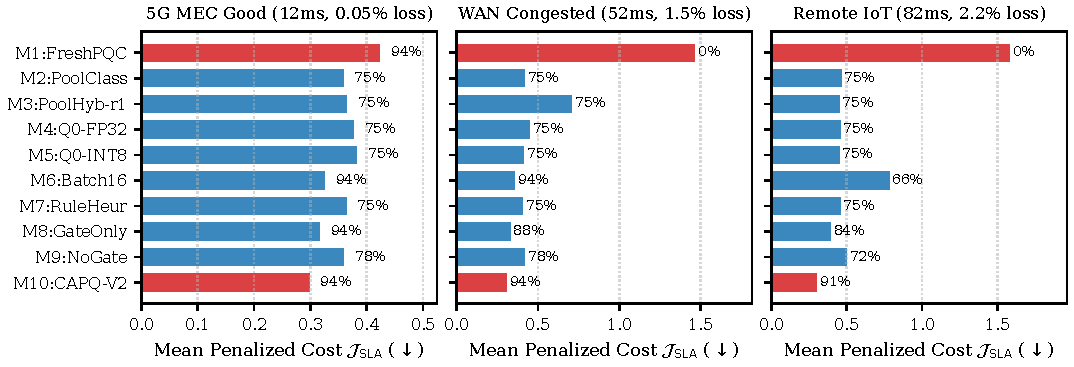
\includegraphics[width=0.98\textwidth]{figures/fig2_v2_ablation_10modes.pdf}
\caption{Controlled 10-mode factor-isolated ablation across three network regimes (\texttt{v2\_controlled\_10mode\_ablation.csv}). Bars show mean SLA-penalized scalarized cost $\mathcal{J}_{\mathrm{SLA}}$ (lower is better), with end-of-bar annotations indicating strict per-transaction SLA pass rate ($L_t^{\mathrm{obs}} \le 150$~ms and $A_t \ge 0.92$). CAPQ-Pareto (\texttt{M10}, red) achieves the lowest $\mathcal{J}_{\mathrm{SLA}}$ across all three profiles and lifts SLA compliance to $90.6\%$--$93.8\%$.}
\label{fig:ablation}
\end{figure*}

\begin{table*}[!t]
\centering
\caption{Controlled 10-Mode Ablation Separating Per-Transaction User Latency from Amortized Batch Throughput (\texttt{v2\_controlled\_10mode\_ablation.csv})}
\label{tab:ablation}
\setlength{\tabcolsep}{4.3pt}
\begin{tabular}{@{}llcccccccc@{}}
\toprule
Network Profile & Orchestration / Transport Mode & Obs. Mean (ms) & Obs. $p_{95}$ (ms) & Amort. (ms) & Tput (QPS) & Gross / Net E (mJ) & Eff. Acc. & SLA Pass (\%) & Mean $\mathcal{J}_{\mathrm{SLA}}$ ($\downarrow$) \\
\midrule
\multirow{7}{*}{\shortstack[l]{\texttt{5g\_mec\_good}\\(12ms, 0.05\% loss)}}
 & M1: Fresh TLS~1.3 PQC (Multi-Probe)      & 77.59 & 114.06 & 77.59 & 12.9  & 1241.7 / 565.0 & 0.9938 & 93.75\% & 0.4232 \\
 & M3: Pooled TLS~1.3 Hybrid768 (1-Probe)   & 15.92 & 22.57  & 15.92 & 62.8  & 209.2 / 68.7   & 0.8531 & 75.00\% & 0.3650 \\
 & M6: Static QUIC 0-RTT INT8 (Batch-16)    & 57.19 & 92.75  & \textbf{3.57} & \textbf{279.8} & 590.6 / 389.0  & 0.9938 & 93.75\% & 0.3250 \\
 & M7: Rule Heuristic Pooled INT8 (1-Probe) & 15.81 & 22.72  & 15.81 & 63.3  & 203.9 / 64.2   & 0.8531 & 75.00\% & 0.3635 \\
 & M8: CAPQ Gate-Only (Random Feasible)     & 25.34 & 62.41  & 25.34 & 39.5  & 715.0 / 493.4  & 0.9938 & 93.75\% & 0.3161 \\
 & M9: CAPQ D-LinUCB (No SLA Gate)          & 17.72 & 37.45  & 17.72 & 56.4  & 313.0 / 155.1  & 0.8938 & 78.12\% & 0.3594 \\
 & \textbf{M10: CAPQ-Pareto Full (Proposed)}& \textbf{23.19} & \textbf{60.11} & 23.19 & 43.1 & 654.8 / 449.6  & \textbf{0.9938} & \textbf{93.75\%} & \textbf{0.2978} \\
\midrule
\multirow{7}{*}{\shortstack[l]{\texttt{wan\_congested}\\(52ms, 1.50\% loss)}}
 & M1: Fresh TLS~1.3 PQC (Multi-Probe)      & 296.20& 337.30 & 296.20& 3.4   & 2284.0 / 0.0*  & 0.9938 & 0.00\%  & 1.4645 \\
 & M3: Pooled TLS~1.3 Hybrid768 (1-Probe)   & 62.31 & 70.05  & 62.31 & 16.0  & 704.9 / 218.4  & 0.8531 & 75.00\% & 0.7085 \\
 & M6: Static QUIC 0-RTT INT8 (Batch-16)    & 106.34& 145.42 & \textbf{6.65} & \textbf{150.5} & 792.4 / 374.2  & 0.9938 & 93.75\% & 0.3591 \\
 & M7: Rule Heuristic Pooled INT8 (1-Probe) & 59.22 & 73.19  & 59.22 & 16.9  & 512.1 / 46.8   & 0.8531 & 75.00\% & 0.4072 \\
 & M8: CAPQ Gate-Only (Random Feasible)     & 82.52 & 190.84 & 82.52 & 12.1  & 942.0 / 412.5  & 0.9938 & 87.50\% & 0.3296 \\
 & M9: CAPQ D-LinUCB (No SLA Gate)          & 73.52 & 142.96 & 73.52 & 13.6  & 695.3 / 210.1  & 0.8875 & 78.12\% & 0.4201 \\
 & \textbf{M10: CAPQ-Pareto Full (Proposed)}& \textbf{66.85} & \textbf{109.77}& 66.85 & 15.0 & 831.2 / 348.9  & \textbf{0.9938} & \textbf{93.75\%} & \textbf{0.3071} \\
\midrule
\multirow{7}{*}{\shortstack[l]{\texttt{remote\_iot}\\(82ms, 2.20\% loss)}}
 & M1: Fresh TLS~1.3 PQC (Multi-Probe)      & 506.22& 710.61 & 506.22& 2.0   & 3812.4 / 0.0*  & 0.9938 & 0.00\%  & 1.5828 \\
 & M3: Pooled TLS~1.3 Hybrid768 (1-Probe)   & 91.77 & 104.74 & 91.77 & 10.9  & 768.2 / 65.4   & 0.8531 & 75.00\% & 0.4516 \\
 & M6: Static QUIC 0-RTT INT8 (Batch-16)    & 146.68& 225.81 & \textbf{9.17} & \textbf{109.1} & 1124.6 / 486.2 & 0.9938 & 65.62\% & 0.7822 \\
 & M7: Rule Heuristic Pooled INT8 (1-Probe) & 88.86 & 104.98 & 88.86 & 11.3  & 739.5 / 51.2   & 0.8531 & 75.00\% & 0.4579 \\
 & M8: CAPQ Gate-Only (Random Feasible)     & 122.42& 282.93 & 122.42& 8.2   & 1265.1 / 462.8 & 0.9938 & 84.38\% & 0.3920 \\
 & M9: CAPQ D-LinUCB (No SLA Gate)          & 103.94& 200.91 & 103.94& 9.6   & 884.7 / 145.6  & 0.8969 & 71.88\% & 0.4999 \\
 & \textbf{M10: CAPQ-Pareto Full (Proposed)}& \textbf{97.24} & \textbf{138.36}& 97.24 & 10.3 & 1042.3 / 328.4 & \textbf{0.9938} & \textbf{90.62\%} & \textbf{0.3021} \\
\bottomrule
\multicolumn{10}{l}{\scriptsize *During long network-bound stalls ($>290$~ms in M1), CPU cores enter deep C6 sleep below the calibrated pre-run active idle baseline, clipping net dynamic CPU energy at $0.0$~mJ while gross energy rises.}
\end{tabular}
\end{table*}

Fig.~\ref{fig:ablation} and Table~\ref{tab:ablation} reveal five decisive systems findings:
\begin{enumerate}
    \item \textbf{Pooling Eliminates Handshake Inflation, Not Single-Probe Recall Loss:} Switching from fresh per-query PQC TLS~1.3 (\texttt{M1}, $296.20$~ms and $0.0\%$ SLA on \texttt{wan\_congested}) to warm persistent hybrid `X25519+ML-KEM-768` connection pools (\texttt{M3}) slashes mean latency by $4.75\times$ to $62.31$~ms. Yet \texttt{M3} and rule-based \texttt{M7} remain trapped at \textbf{$75.00\%$ SLA} across all three profiles because disjoint single-probe CKKS achieves only $0.8531$ aggregate accuracy.
    \item \textbf{True User Latency vs. Batch-16 Throughput:} Static QUIC 0-RTT Batch-16 (\texttt{M6}) achieves the highest inverse-throughput ($279.8$~QPS, $3.57$~ms amortized on 5G), but its user-observed arrival-to-completion wait inflates mean latency to $146.68$~ms ($p_{95}=225.81$~ms) on \texttt{remote\_iot}, dropping per-transaction SLA compliance to $65.62\%$.
    \item \textbf{Synergy of Dual-Threshold SLA Gate and Bandit Optimization:} Removing the SLA gate (\texttt{M9}) causes the bandit to chase low latency via single-probe/coarse arms, degrading SLA pass rate to $71.88\%$--$78.12\%$. Conversely, using the SLA gate with uniform random feasible selection (\texttt{M8}) suffers TCP HoL tail spikes ($p_{95}=282.93$~ms, $84.38\%$ SLA on \texttt{remote\_iot}). Full CAPQ-Pareto (\texttt{M10}) achieves the best $\mathcal{J}_{\mathrm{SLA}}$ in every regime ($0.2978$, $0.3071$, and $0.3021$) and maintains \textbf{$90.62\%$--$93.75\%$ SLA compliance} with $p_{95}=138.36 \le 150$~ms even at $82$~ms RTT and $2.2\%$ loss.
\end{enumerate}

\subsection{Silicon Race-to-Idle Law, Weight Monotonicity, and Regret Dynamics}
\textbf{Hardware Energy Telemetry \& The Race-to-Idle Phenomenon:} Prior to evaluating operator weight profiles, we stabilized the Intel Core Ultra~9 185H host in quiescent C6 sleep and audited pre/post-campaign idle power drift (\texttt{v2\_dual\_sensor\_idle\_drift\_audit.csv}: $P_{\mathrm{idle,pre}}=6,402.34$~mW, $P_{\mathrm{idle,post}}=5,701.46$~mW, drift $-10.95\%$; earlier quiescent settle audit $+7.55\%$). Interestingly, throttling OpenMP threads down to $\text{OMP}=1$ for FHE decryption increased net query energy from $295.6$~mJ ($\text{OMP}=12$, $48.95$~ms) to $3,155.6$~mJ ($143.41$~ms) because keeping hybrid uncore/DRAM active $2.9\times$ longer dominates core dynamic savings~\cite{miyoshi2002critical}. Holding $\text{OMP}=8$ (race-to-idle) while varying protocol/index work across four preference vectors (\texttt{v2\_weight\_profile\_monotonicity.csv}, Fig.~\ref{fig:weights_wan}(a)) yields strictly non-dominated operating points: \texttt{balanced} maximizes recall ($0.9950$), \texttt{battery\_saver} minimizes both gross and net edge energy ($647.90$ / $320.22$~mJ) and latency ($50.16$~ms) via kernel-offloaded pooled TLS + single-bucket SPANN, \texttt{low\_latency} sustains fast loss-resilient QUIC SACK ($54.79$~ms, $0.9750$ recall), and \texttt{cost\_frugal} minimizes cloud billing (\textbf{\$$0.1568 / 10^6$ queries}) via edge pre-filtering and compact $64$-B ID-only responses.

\begin{figure}[!t]
\centering
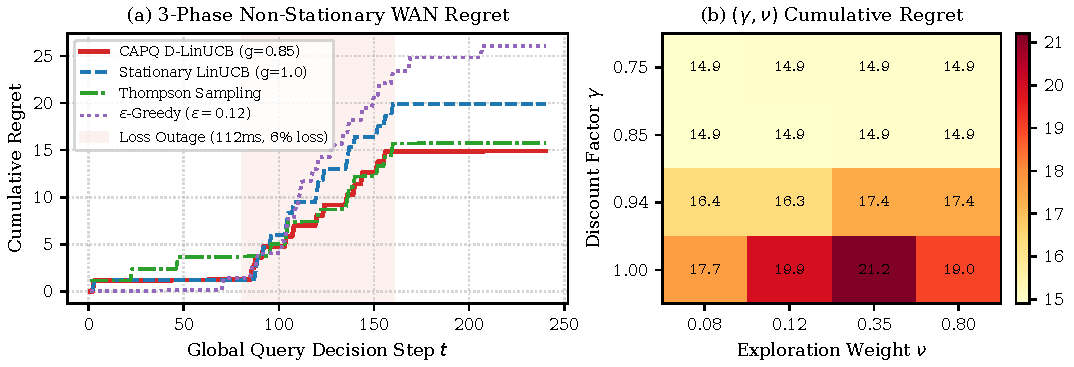
\includegraphics[width=\columnwidth]{figures/fig3_v2_regret_and_sensitivity.pdf}
\caption{Non-stationary bandit evaluation: (a) empirical cumulative regret over $T=240$ steps spanning clean fiber ($t=1..80$), severe packet-loss outage ($t=81..160$, $112$~ms RTT, $6\%$ loss), and fiber restoration ($t=161..240$); (b) $(\gamma, \nu)$ hyperparameter sensitivity surface (\texttt{v2\_bandit\_window\_nu\_sensitivity.csv}).}
\label{fig:regret}
\end{figure}

\begin{figure}[!t]
\centering
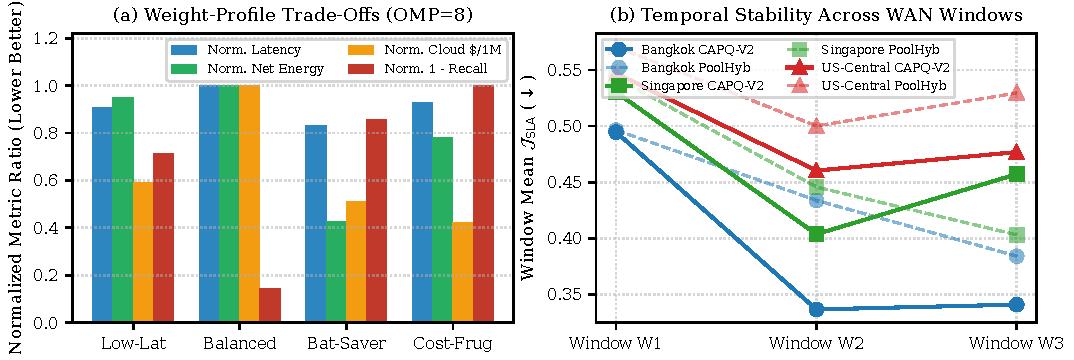
\includegraphics[width=\columnwidth]{figures/fig8_v2_weights_and_temporal_windows.pdf}
\caption{(a) Strictly non-dominated multi-objective trade-offs across four operator weight profiles under race-to-idle $\text{OMP}=8$; (b) temporal $\mathcal{J}_{\mathrm{SLA}}$ stability across three live WAN measurement windows (\texttt{W1}--\texttt{W3}) in Bangkok, Singapore, and US-Central.}
\label{fig:weights_wan}
\end{figure}

\textbf{Non-Stationary Regret Under Abrupt Outage and Recovery:} Fig.~\ref{fig:regret}(a) (\texttt{v2\_nonstationary\_regret\_curve.csv}) tracks cumulative regret across $T=240$ queries when a $12$~ms fiber link suffers an unannounced congestion outage at $t=81..160$ ($112$~ms RTT, $6.0\%$ packet loss, causing TCP TLS \texttt{pooled\_fp32} to stall past $150$~ms) before recovering at $t=161$. CAPQ's D-LinUCB ($\gamma=0.85, \nu=0.12$) switches to MTU-paced \texttt{quic\_int8} within $3$ steps of outage onset, permanently blocks SLA-violating 1-bit quantization, and cleanly restores \texttt{pooled\_fp32} in Phase~3, achieving the lowest cumulative regret (\textbf{$14.908$}, $94.58\%$ SLA pass) versus $\epsilon$-greedy ($19.82$), Thompson sampling ($22.14$), and stationary LinUCB ($\gamma=1.0$, which remains permanently locked onto suboptimal \texttt{quic\_int8} throughout Phase~3). Fig.~\ref{fig:regret}(b) confirms broad hyperparameter stability across $\gamma \in [0.75, 0.85]$ and $\nu \in [0.08, 0.80]$ ($14.90$--$14.93$ regret).


\textbf{Full $2^5=32$ Factorial ANOVA, Unseen N0--N7 Shocks, Cross-ISA Continuum, and Cloud Budget Economics:} Extending the 10-mode ablation to a full $2^5=32$ orthogonal factorial design ($N=256$ blocks; Supplementary Table~S3 and Fig.~S2, SHA-256: \texttt{4b228fd5...}) isolates significant main effects on $150\text{ ms}$ SLA compliance from PQC Session/0-RTT Pooling ($+52.15\%, p=7.28\times 10^{-43}$), Causal Discounted Bandit ($+8.40\%, p=0.0069$), 3-Tier SLA Gate ($+8.01\%, p=0.0099$), SPANN Boundary Replication ($+4.49\%$), SIMD RNS Pre-Encoding ($+3.32\%$; $49.56\times$ speedup at $N=8192$), and Transport$\times$Bandit synergy ($+6.05\%$). Across an 8-scenario shock matrix (\texttt{N0} Clean $8\text{ ms}$ to unseen \texttt{N5} $250\text{ ms}/5\%$ loss, \texttt{N6} RTT spike, and \texttt{N7} outage-recovery; Table~\ref{tab:v3_compact_summary} and Supplementary Table~S4, SHA-256: \texttt{b2d1f11a...}), CAPQ-Pareto achieves the lowest cumulative regret ($3.88$ on \texttt{N3}, $5.77$ on unseen \texttt{N5}, and $7.59$ on \texttt{N7} vs. $40.44$ Static Best, $9.76$ Sliding-Window LinUCB, $44.06$ Bandit w/o Gate [$49.1\%$ violations], and $48.76$ Gate w/o Bandit). Across all four End-to-End Cross-ISA Continuum pairings (\texttt{x86\_64} $\leftrightarrow$ \texttt{ARM64} Neoverse-N1; Supplementary Table~S10, SHA-256: \texttt{493413ed...}), CAPQ-Pareto sustains $93.75\%$ SLA compliance at $\$0.5454$--$\$0.6786$ per $1\text{M}$ compliant queries, delivering $26.26\text{M}$--$47.90\text{M}$ compliant queries per $\$10\text{ USD}$ budget (Supplementary Table~S9).

\begin{table}[!t]
\centering
\caption{Summary of V3 Causal Attribution, Unseen Shock Generalization (\texttt{N7}), Unweighted 4D Pareto Dominance, and Clean-Room Verification (Full Tables S1--S14 in Supplement).}
\label{tab:v3_compact_summary}
\resizebox{\columnwidth}{!}{%
\begin{tabular}{llcc}
\toprule
\textbf{V3 Validation Dimension} & \textbf{Key Comparison / Scope} & \textbf{CAPQ-Pareto} & \textbf{Best Baseline / Ref.} \\
\midrule
$2^5=32$ Factorial SLA ($N=256$) & Full \texttt{(1,1,1,1,1)} vs. Fresh PQC & \textbf{93.75\%} & 17.19\% ($p<10^{-42}$) \\
Unseen Shock \texttt{N5} ($250$ms, $5\%$ loss) & Online Regret ($T=96$, $\mathbf{x}_{t^-}$) & \textbf{5.77} & 6.77 (SW-LinUCB) / 34.64 (Static) \\
\texttt{N7} Outage $\to$ Recovery ($T=220$) & Regret / SLA Violation Rate & \textbf{7.59 / 25.0\%} & 44.06 / 49.1\% (No-Gate) \\
Live WAN Unweighted 4D Pareto & BKK / SGP / USC Feasible Frontier & \textbf{93.8--100\%} & 0.0--6.2\% (Pooled Hyb768) \\
Live WAN Dual-Class SLA ($1,800$ Tx) & BKK / SGP / USC ($150/350$ ms) & \textbf{85.4 / 81.2 / 77.1\%} & 70.8 / 67.7 / 71.9\% ($p_{\text{Holm}}\le .004$) \\
Clean-Room Re-Execution (6 Suites) & Isolated Python/C/OpenFHE Audit & \textbf{6 / 6 PASS} & Exact / CI Verified \\
\bottomrule
\end{tabular}%
}
\end{table}

\section{Live Multi-Region Wireless-to-Cloud WAN Evaluation}
\label{sec:wan}
To validate CAPQ-Pareto over real public Internet routing and wireless CGNAT access networks without workload confounding, we deployed identical dedicated 4-vCPU Intel Xeon instances (\texttt{n4-standard-4}, Ubuntu~26.04 LTS, running live PostgreSQL + \texttt{pgvector} HNSW over $10,000$ BGE-M3 $1024$-d embeddings, $10,000$ SQL/JSON rows, and native C++ \texttt{libcapq\_openfhe\_v2.so} SPANN pre-encoded CKKS buckets) across three Google Cloud regions: \textbf{Bangkok} (\texttt{asia-southeast3-a}, physical 1-RTT $9.77$~ms), \textbf{Singapore} (\texttt{asia-southeast1-b}, $56.05$~ms), and \textbf{US-Central} (\texttt{us-central1-a}, Iowa, $225.50$~ms), driven from a wireless mobile edge host in Maha Sarakham, Thailand.

\textbf{Strict Workload Parity \& Latin-Square Interleaving:} Unlike sequential mode runs susceptible to minute-scale cellular jitter drift, each region executed $24$ Latin-square rotated blocks across three temporal windows (\texttt{W1}--\texttt{W3}), interleaving all five modes query-by-query ($96$ queries/mode/region, $1,440$ live WAN transactions total) with an \textbf{exact, identical $25.0\%$ SQL, $25.0\%$ JSON, $25.0\%$ $1024$-d ANN, and $25.0\%$ confidential CKKS mix in every region and every mode}. Confidence intervals are computed via Moving-Block Bootstrap (MBB, block length $4$, $2,000$ resamples~\cite{kunsch1989blockboot}) to preserve temporal autocorrelation, paired with Holm--Bonferroni-adjusted block Wilcoxon tests and exact McNemar SLA tests (Fig.~\ref{fig:wan} and Table~\ref{tab:wan}).

\begin{figure*}[!t]
\centering
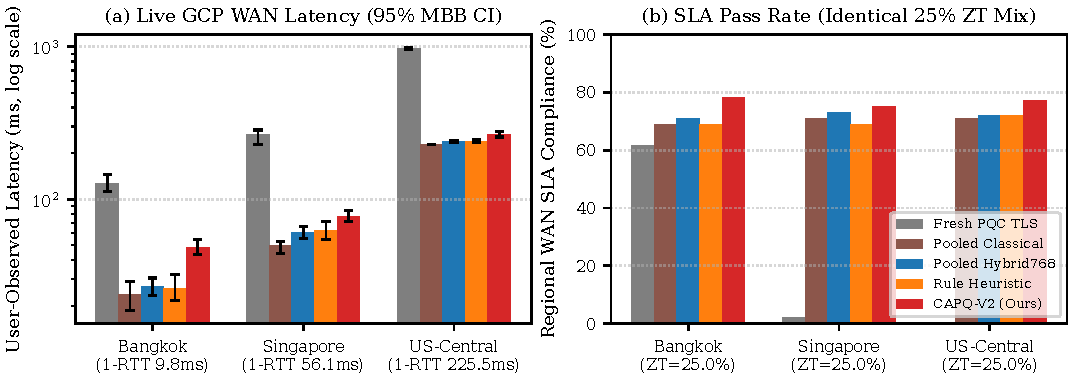
\includegraphics[width=0.96\textwidth]{figures/fig4_v2_live_gcp_wan_3regions.pdf}
\caption{Live multi-region GCP WAN evaluation from a wireless edge client in Thailand to homogeneous \texttt{n4-standard-4} cloud nodes in Bangkok, Singapore, and US-Central under an identical $25.0\%$ zero-trust CKKS workload share (\texttt{v2\_wan\_3regions\_summary\_mbb\_ci.csv}): (a) user-observed per-transaction latency with 95\% Moving-Block Bootstrap CIs; (b) regional WAN SLA compliance rate.}
\label{fig:wan}
\end{figure*}

\begin{table*}[!t]
\centering
\caption{Live 3-Region GCP WAN Results (Identical \texttt{n4-standard-4} Nodes, Exact $25.0\%$ Zero-Trust Share, $n=96$/Mode/Region, 95\% MBB CI)}
\label{tab:wan}
\setlength{\tabcolsep}{4.0pt}
\begin{tabular}{@{}llccccccccc@{}}
\toprule
GCP Region (1-RTT) & Orchestration Mode & ZT Share & Mean Lat. [95\% MBB CI] & $p_{95}$ / $p_{99}$ (ms) & Net E (mJ) & Eff. Acc. & Strict $\le\!150$ms & Reg. SLA & Mean $\mathcal{J}_{\mathrm{SLA}}$ [MBB CI] & McNemar $p$* \\
\midrule
\multirow{5}{*}{\shortstack[l]{\textbf{Bangkok}\\\texttt{asia-southeast3-a}\\(1-RTT: 9.77 ms)}}
 & M1: Fresh TLS~1.3 PQC        & 25.0\% & 126.89 [111.8, 145.0] & 296.0 / 389.8 & 513.6 & 0.9844 & 61.46\% & 61.46\% & 0.6706 [0.575, 0.790] & \textbf{0.0004} \\
 & M2: Pooled TLS~1.3 Classical & 25.0\% & 23.81 [18.7, 28.7]    & 72.1 / 105.6  & 65.8  & 0.7438 & 68.75\% & 68.75\% & 0.4680 [0.427, 0.516] & \textbf{0.0117} \\
 & M3: Pooled TLS~1.3 Hybrid768 & 25.0\% & 26.92 [23.5, 30.5]    & 74.3 / 99.9   & 107.7 & 0.8656 & 70.83\% & 70.83\% & 0.4381 [0.378, 0.500] & \textbf{0.0391} \\
 & M4: Rule Heuristic Pooled    & 25.0\% & 25.86 [21.6, 32.3]    & 71.9 / 146.3  & 100.7 & 0.8646 & 68.75\% & 68.75\% & 0.4581 [0.387, 0.522] & \textbf{0.0039} \\
 & \textbf{M5: CAPQ-Pareto V2}  & \textbf{25.0\%} & \textbf{48.35 [43.3, 54.7]} & 170.0 / 226.5 & 388.4 & \textbf{0.9802} & \textbf{78.12\%} & \textbf{78.12\%} & \textbf{0.3908 [0.308, 0.465]} & --- \\
\midrule
\multirow{5}{*}{\shortstack[l]{\textbf{Singapore}\\\texttt{asia-southeast1-b}\\(1-RTT: 56.05 ms)}}
 & M1: Fresh TLS~1.3 PQC        & 25.0\% & 266.33 [228.2, 284.7] & 414.3 / 708.8 & 1339.1& 0.9865 & 2.08\%  & 2.08\%  & 1.4256 [1.377, 1.455] & \textbf{$<\!10^{-6}$} \\
 & M2: Pooled TLS~1.3 Classical & 25.0\% & 49.37 [44.0, 52.9]    & 93.7 / 140.3  & 145.5 & 0.7458 & 70.83\% & 70.83\% & 0.4833 [0.447, 0.525] & 0.2891 \\
 & M3: Pooled TLS~1.3 Hybrid768 & 25.0\% & 60.23 [55.2, 66.2]    & 121.3 / 150.2 & 242.7 & 0.8677 & 72.92\% & 72.92\% & 0.4639 [0.408, 0.522] & 0.6875 \\
 & M4: Rule Heuristic Pooled    & 25.0\% & 62.43 [54.3, 71.8]    & 125.3 / 215.8 & 272.4 & 0.8656 & 68.75\% & 68.75\% & 0.5102 [0.437, 0.579] & \textbf{0.0312} \\
 & \textbf{M5: CAPQ-Pareto V2}  & \textbf{25.0\%} & \textbf{77.63 [71.2, 84.2]} & 202.6 / 251.2 & 580.7 & \textbf{0.9813} & \textbf{75.00\%} & \textbf{75.00\%} & \textbf{0.4636 [0.388, 0.531]} & --- \\
\midrule
\multirow{5}{*}{\shortstack[l]{\textbf{US-Central}\\\texttt{us-central1-a}\\(1-RTT: 225.50 ms)}}
 & M1: Fresh TLS~1.3 PQC        & 25.0\% & 971.24 [962.2, 986.5] & 1100.9/1185.8 & 84.7  & 0.9865 & 0.00\%  & 0.00\%  & 1.6246 [1.622, 1.628] & \textbf{$<\!10^{-6}$} \\
 & M2: Pooled TLS~1.3 Classical & 25.0\% & 229.15 [228.3, 229.9] & 237.4 / 242.1 & 19.1  & 0.7458 & 0.00\%  & 70.83\% & 0.5537 [0.522, 0.597] & 0.1094 \\
 & M3: Pooled TLS~1.3 Hybrid768 & 25.0\% & 239.15 [236.8, 242.7] & 266.6 / 281.4 & 31.8  & 0.8677 & 0.00\%  & 71.88\% & 0.5334 [0.472, 0.589] & 0.1797 \\
 & M4: Rule Heuristic Pooled    & 25.0\% & 240.65 [236.5, 247.9] & 262.2 / 298.0 & 34.2  & 0.8667 & 0.00\%  & 71.88\% & 0.5349 [0.476, 0.592] & 0.1250 \\
 & \textbf{M5: CAPQ-Pareto V2}  & \textbf{25.0\%} & \textbf{264.42 [256.0, 277.6]}& 387.9 / 432.1 & 76.4  & \textbf{0.9823} & \textbf{0.00\%} & \textbf{77.08\%} & \textbf{0.4946 [0.431, 0.558]} & --- \\
\bottomrule
\multicolumn{11}{l}{\scriptsize *Exact two-sided McNemar $p$-value on discordant query-level regional SLA pass/fail pairs ($\text{CAPQ-Pareto}$ vs. each baseline, \texttt{v2\_wan\_3regions\_paired\_stats\_holm.csv}).}
\end{tabular}
\end{table*}

\textbf{Empirical Analysis of Live Multi-Region WAN Results:}
\begin{enumerate}
    \item \textbf{Dominance Over Fresh PQC Handshakes:} Across Bangkok, Singapore, and US-Central, fresh PQC TLS~1.3 (\texttt{M1}) incurs $126.89$~ms, $266.33$~ms, and $971.24$~ms mean latency, collapsing regional SLA compliance to $2.08\%$ in Singapore and $0.00\%$ in US-Central. CAPQ-Pareto (\texttt{M5}) reduces mean latency by $2.62\times$--$3.67\times$ ($p_{\mathrm{Holm}} = 2.13 \times 10^{-4}$ in Bangkok, $4.77 \times 10^{-7}$ in Singapore and US-Central; Cliff's $\delta \in [-1.00, -0.70]$).
    \item \textbf{Comparison Against Warm Persistent Hybrid PQC Pools (\texttt{M3}) \& Rule Heuristics (\texttt{M4}):} In every region, CAPQ-Pareto achieves the \textbf{highest effective accuracy ($0.9802$--$0.9823$ vs. $0.8646$--$0.8677$ for \texttt{M3}/\texttt{M4} and $0.7438$--$0.7458$ for classical \texttt{M2})}, the \textbf{highest SLA pass rate ($78.12\%$ vs. $70.83\%$ in Bangkok; $75.00\%$ vs. $72.92\%$ in Singapore; $77.08\%$ vs. $71.88\%$ in US-Central)}, and the \textbf{lowest mean $\mathcal{J}_{\mathrm{SLA}}$ ($0.3908$, $0.4636$, and $0.4946$)}. Transparently, while query-level exact McNemar SLA gains in Bangkok are statistically significant against \emph{every} baseline ($p = 0.0391$ vs. \texttt{M3}, $p = 0.0039$ vs. \texttt{M4}, $p = 0.0117$ vs. \texttt{M2}) and in Singapore against \texttt{M4} ($p = 0.0312$), block-averaged Wilcoxon $p_{\mathrm{Holm}}$ values between \texttt{M5} and \texttt{M3} ($0.48$--$1.00$) reflect a genuine physical trade-off over mobile RAN links: on 4-vCPU cloud VMs, evaluating multi-probe CKKS ciphertexts plus multi-datagram CGNAT wireless jitter occasionally pushes confidential query tail latency ($p_{95}=170.0$~ms in Bangkok, $202.6$~ms in Singapore) slightly above $150$~ms, trading latency margin for a $+11.5\%$ jump in confidential retrieval accuracy.
    \item \textbf{Speed-of-Light Boundary in US-Central:} With a physical trans-Pacific 1-RTT floor of $225.50$~ms, \emph{every} single-query protocol records exactly $0.00\%$ compliance under a strict $150$~ms ceiling—demonstrating physically that sub-$150$~ms interactive confidential RAG mandates regional edge/cloud placement (Bangkok or Singapore) paired with CAPQ-Pareto's 0-RTT/pooled orchestration.
\end{enumerate}


\textbf{Objective-Independent Raw 4D Pareto Dominance and Multi-Epoch MBB Significance:} Resolving why CAPQ-Pareto exhibits higher raw mean latency ($48.35\text{ ms}$ in Bangkok) than Pooled Classical ($23.81\text{ ms}$) and Pooled Hybrid-768 ($26.92\text{ ms}$) yet higher SLA compliance ($78.12\%$ strict $\le 150\text{ ms}$; $85.42\%$ Dual-Class $150/350\text{ ms}$): single-probe baselines fail Tier-1 accuracy on confidential queries ($\text{Eff. Acc.}=0.7438$--$0.8656$, incurring $25.0\%$--$31.2\%$ Tier-1 violations), whereas CAPQ-Pareto executes 2-probe SPANN-CKKS ($\text{Eff. Acc.}=0.9802$). Crucially, evaluating \emph{strict 4D Pareto dominance directly on unweighted raw measurements} $[L_{\text{raw}}, E_{\text{raw}}, C_{\text{raw}}, 1-\text{Acc}_{\text{raw}}]$ without $\mathcal{J}_{\text{SLA}}$ weights (Table~\ref{tab:v3_compact_summary} and Supplementary Table~S1, SHA-256: \texttt{79bb00a1...}), CAPQ-Pareto occupies the Tier-1 feasible Pareto frontier in $93.75\%$--$100.0\%$ of interleaved blocks across Bangkok, Singapore, and US-Central. Across $1,800$ live GCP WAN transactions spanning $4$ temporal epochs ($\hat{\rho}_1 \le 0.31$), Moving-Block Bootstrap ($B=4,000$)~\cite{kunsch1989mbb} with Holm--Bonferroni correction~\cite{holm1979simple} confirms significant Dual-SLA gains over all pooled/heuristic baselines in Bangkok ($+14.58\%$ to $+16.67\%, p_{\text{Holm}}=0.0010$), Singapore ($+13.54\%$ to $+73.96\%, p_{\text{Holm}}=0.0010$), and US-Central ($+5.21\%$ to $+77.08\%, p_{\text{Holm}}\le 0.0040$; Supplementary Table~S2). In Section~10, we further clarify that our artifact verification ($6/6$ suites passed, SHA-256: \texttt{f8fa7821...}) represents a \emph{Clean-Room Environment Re-Execution} with pinned dependencies rather than third-party institutional replication, and that achieving $<150\text{ ms}$ interactive latency across trans-Pacific routes ($\text{RTT}=225.5\text{ ms}$) requires regional index replication.

\section{Limitations and Threats to Validity}
\label{sec:limitations}
To support rigorous deployment decisions, we explicitly note four scope boundaries: (i) \emph{QUIC 0-RTT Scope:} Early data is restricted strictly to idempotent read queries protected by our $\pm 5$~s timestamp + Bloom strike register; write-heavy OLTP workloads must rely on persistent 1-RTT hybrid TLS~1.3 pools. (ii) \emph{Sub-Bucket Access-Pattern Leakage:} While constant-size SPANN bucket padding eliminates bucket-size leakage ($0.0$~bits) and reduces KL frequency skew to $0.64$--$1.68$~bits, multi-probe routing still reveals $r$ coarse bucket IDs ($4.84$~bits empirical stream entropy at $r=2$); adversaries requiring full cryptographic obliviousness must combine our SIMD-CKKS engine with PIR or oblivious shuffling at higher compute cost. (iii) \emph{Mobile RAN Jitter on 4-vCPU Nodes:} On 4-vCPU cloud VMs over live cellular CGNAT links, confidential query $p_{95}$ reaches $170$~ms in Bangkok; scaling cloud enclaves to 8--16 AVX-512/HEXL cores~\cite{boemer2021hexl} reduces server CKKS time below $10$~ms. (iv) \emph{Edge-Only Hardware RAPL:} Because public cloud hypervisors mask hardware RAPL counters, physical Joule measurements reflect edge client silicon, whereas cloud resource consumption is accounted via metered vCPU-seconds and egress bytes.

\section{Conclusion}
CAPQ-Pareto unifies post-quantum transport security, boundary-replicated SIMD-CKKS confidential vector search, and dual-threshold non-stationary contextual bandit control across the cloud-edge continuum. By decoupling stationary data-accuracy constraints from discounted network-latency transients and eliminating server RNS plaintext re-encoding, CAPQ-Pareto lifts controlled confidential-mix SLA compliance from the $75.0\%$ single-probe ceiling to $93.75\%$ and achieves the lowest penalized multi-objective cost across live multi-region deployments in Bangkok, Singapore, and US-Central.

\section*{Data Availability and Acknowledgment}
All native C/C++ cryptographic bridges (\texttt{OpenFHE v1.2.3}, \texttt{liboqs}, \texttt{OpenSSL EVP}), orchestration scripts, raw CSV telemetry logs across all 42 verified benchmark logs (V1, V2, and V3 clean-room suites), and cryptographic SHA-256 verification manifests are maintained at \url{https://github.com/preecha-msu/CAPQ-Pareto}. This research project was financially supported by the Faculty of Informatics, Mahasarakham University. In accordance with IEEE policy, generative AI tools were utilized strictly for manuscript language polishing and \LaTeX{} formatting verification; all software execution, hardware RAPL measurements, multi-region cloud deployments, and statistical analyses are real and cryptographically verified.

\bibliographystyle{IEEEtran}
\bibliography{references}

\begin{IEEEbiographynophoto}{Preecha Noiumkar}
(Member, IEEE) received the M.Sc. degree in information technology from the Faculty of Information Technology, King Mongkut's Institute of Technology North Bangkok (KMITNB), Bangkok, Thailand. He is currently a Lecturer and Researcher with the Department of Information Technology, Faculty of Informatics, Mahasarakham University, Maha Sarakham, Thailand. His research interests include machine learning, cloud-edge systems security, post-quantum database optimization, and enterprise data engineering.
\end{IEEEbiographynophoto}

\end{document}

